%!TEX root = ../thesis.tex
%*******************************************************************************
%*********************************** First Chapter *****************************
%*******************************************************************************

\chapter{Introduction}  %Title of the First Chapter
\pagebreak
%s\doublespacing
\onehalfspacing

\section{Overview}

All organisms exist in a state of intense competition for resources. For many organisms, among the most dangerous competitors are parasites, which attempt to colonise the host's own body and co-opt its internal resources and systems to their own advantage. The evolutionary arms race between parasites and hosts is ancient, and has led to the development of a stunning variety of complex offensive and defensive adaptations on each side. % Mention faster evolution of parasites relative to hosts

Among the most complex and sophisticated systems developed as part of this ancient host/parasite conflict is the vertebrate adaptive immune system. By dynamically recombining their own DNA within specialised lymphocyte cells, jawed vertebrates are capable of producing an almost unlimited variety of different \textit{de novo} antigen-receptor proteins, and hence of responding effectively to entirely novel immune threats. In addition, by producing long-lived memory cells in response to antigenic stimulation, the adaptive immune system can retain the ability to respond to recurrent immune threats years or even decades after they were first encountered by an individual. This combination of dynamic adaptability to novel immune threats and persistent immune memory enables vertebrates to progressively improve their protection against predictable aspects of their immune environment, while also coping effectively with the rapid evolution which is one of the main advantages of bacterial and viral pathogens over their slower-evolving hosts.

Among the different branches of vertebrate adaptive immunity, the humoral immune system is unique in both the breadth of antigenic compounds it can respond to and its ability to produce secreted antigen-receptor proteins capable of acting independently of the cells that produced them. Whereas the T-lymphocytes of the cellular adaptive immune system can respond only to processed peptide antigens expressed on the surface of antigen-presenting cells, the antibodies produced by B-lymphocytes are capable of responding to almost any molecular structure on the surface of a cell or protein. Secreted antibodies in serum and mucosal secretions play a number of essential roles in vertebrate immunity, including opsonisation (recruitment of phagocytic cells), activation of complement, and inactivation and aggregation of antigens and pathogens, while membrane-bound antibodies (also known as B-cell receptors or BCRs) orchestrate B-cell development, and response to antigen exposure. An effective humoral immune system is essential to immune and organismal function in vertebrates, and mutations that disable humoral adaptive immunity in ...% species?
can lead to severe immunopathies and severely curtailed life expectancy. % TODO: Focus on importance here, move details to another section.

% TODO: Discuss antibodies specifically

Despite all its sophistication, however, the functionality of the vertebrate adaptive immune system declines dramatically with age, leaving older individuals increasingly vulnerable to infectious disease. In humans and other species, the decline in immune functionality with age manifests as a dramatic increase in deaths from infection in older people, as well as increasing levels of infection-associated morbidity and a decline in the effectiveness of pro-immune interventions such as vaccination. The molecular and physiological changes underlying this immunosenescent phenotype are wide-ranging, implicating many different parts of the immune system; however, a particularly important contributor is the systemic decline in the effectiveness of the adaptive immune system in % identifying and neutralising novel immune threats?
For the humoral adaptive immune system, established immunosenescent phenotypes include... % decline in naive B-cells, reduction of antibody avidity, increase in autoantibody production
% TODO: Recast in terms of humoral immunity *as part of* general immune phenotype

While fair amount is known about the cellular and physiological changes that take place in the humoral adaptive immune system with age in some species, much less is known about how these changes translate to alterations in the high-level diversity, clonal makeup, and other structural aspects of the overall antibody repertoire in older individuals. Such a high-level systemic approach to antibody diversity could potentially reveal a great deal about how ageing and other processes affect adaptive immune functionality in an organism. Specialised, high-throughput, quantitative approaches have been used to assess the structure, diversity and health of adaptive immune repertoires in various contexts, including development, disease, and ageing; in the latter case, this pre-existing work has revealed ... . However, much remains to be discovered about ... .

When it comes to investigating the ageing of vertebrate-specific adaptations like the adaptive immune system, research is made more difficult by a relative lack of well-suited model organisms. Most established short-lived model organisms used in ageing research (e.g. yeast, nematode worms, or fruit flies) are not vertebrates, while most established vertebrate models (e.g. zebrafish or \species{Xenopus}{laevis}) were selected for properties other than their lifespan (such as rapid development) and are too long-lived for use as ageing models in many contexts. Even mouse, the most widely-used vertebrate model organism for both ageing and other biomedical applications, has a median lifespan of several years in most commonly-used laboratory strains, making many ageing studies prohibitively expensive. 

In this context, the recent emergence of the turquoise killifish (\nfu), the shortest-lived vertebrate species currently bred in captivity, as a model organism for ageing research represents a highly promising development for the study of adaptive immunosenescence; ...

In this thesis, therefore, I establish the turquoise killifish as a model for the study of comparative immunology and humoral adaptive immunosenescence. 
, by characterising 

Using a combination of existing genomic assemblies and new sequence data, I assembled and characterised the immunoglobulin heavy chain (\igh{}) gene locus of the turquoise killifish and compared it to other newly-assembled loci from closely-related species, revealing a complex and rapidly-evolving ... with a number of surprisingly ideosyncratic features (\Cref{chap:locus}). Using the sequences from this newly-characterised locus, I established the first working immunoglobulin sequencing protocol in this species, which I used to investigate the diversity and complexity of heavy-chain immune repertoires in adult killifish and how this diversity changes with age in the whole body and the gut. The results of these investigations demonstrate that the turquoise killifish possesses a complex, diverse and individualised antibody repertoire, which undergoes a rapid decline in within-individual diversity and increase in between-individual variability with age. This phenomenon is particularly strong in the gut, with ..., and is likely to be an important contributor to the changes in gut microbiota structure and diversity observed in aged killifish. % TODO: Discuss lack of change from transfer?

\section{The humoral adaptive immune system in jawed vertebrates}

\subsection{Antibody structure and function}
\label{sec:intro_antibody_structure}

The lineage of lymphocytic white blood cells known as B-cells is ancient, with its origins predating any modern jawed-vertebrate lineage and possibly the development of antibodies themselves \parencite{boehm2011design,kasahara2015vlr}. In modern jawed vertebrates, B-lymphocytes are responsible for the production, diversification and secretion of the antigen-receptor proteins known as antibodies \parencite{mix2006immunoglobulins,schroeder2010immunoglobulins}, as well as diverse other roles that vary between taxa \parencite{sunyer2013fishing}. In almost all species examined to date, antibodies share a common, and highly distinctive, tetrameric structure (\Cref{fig:intro-antibody-structure-schematic}), with two identical immunoglobulin heavy chains (IGH) and two light chains (IGL) linked by disulfide bonds into a roughly Y-shaped configuration \parencite{mix2006immunoglobulins,schroeder2010immunoglobulins}. The sequence and structure of these chains, and the corresponding regions of their underlying gene loci, is divided into an N-terminal (5') variable region and a C-terminal (3') constant region \parencite{mix2006immunoglobulins} (\Cref{fig:intro-antibody-structure-schematic}); together, the variable regions of each light/heavy-chain pair determines the antigen-binding specificity of the antibody, while the constant regions, particularly that of the heavy chain, determine its structure, functional properties, and interactions with the rest of the immune system \parencite{mix2006immunoglobulins,schroeder2010immunoglobulins}. Unsurprisingly, the sequence diversity of the constant region is far lower than that of the variable region, with most species expressing only a few distinct constant-region classes (or \textit{isotypes}) but an almost unlimited variety of variable-region sequences (or \textit{ideotypes}).

As members of the immunoglobulin superfamily of proteins, the tertiary structure of antibody chains consists primarily of a species of immunoglobulin fold domains; most light chains consist of two such domains, while the number in heavy chains varies substantially with isotype \parencite{schroeder2010immunoglobulins}. In both heavy and light chains, the most N-terminal immunoglobulin fold comprises the variable region, while the rest make up the constant region (\Cref{fig:intro-antibody-structure-schematic}); in some taxa (but not in teleost fishes), one of the constant-region immunoglobulin folds is replaced with a flexible hinge domain in some isotypes to increase the flexibility of the heavy chain \parencite{schroeder2010immunoglobulins}. The three loops of the protein chain facing the antigen-binding site are labelled H1, H2 and H3 in the heavy chain and L1, L2 and L3 in the light chain (\Cref{fig:intro-antibody-structure-loops}) \parencite{shirai1999h3} and are principally responsible for determining the antigen-binding specificity of the antibody; their corresponding gene regions are known as complementarity-determining regions (CDRs) and are the main focus of sequence variability among ideotypes, while the other parts of the antibody sequence are known as framework regions (FRs or FWRs) and exhibit less variability \parencite{schroeder2010immunoglobulins}.

Most antibody isotypes can be expressed in secreted or membrane-bound form; in the latter case they are also known as B-cell receptors (BCRs) \parencite{bengten2015fishantibodies}. The choice between secreted and membrane-bound forms of an antibody is usually made through alternative splicing \parencite{bengten2015fishantibodies,mashoof2016immunoglobulins}; typically, the transmembrane domain and cytosolic tail of the BCR are expressed via two additional exons (TM1 and TM2). Other constant-region exons are referred to collectively as CH exons, and are numbered by their occurence in the protein chain from the variable region to the C-terminus. In secreted antibodies, the standard four-chain configuration described above is known as an antibody monomer \parencite{mix2006immunoglobulins}, while multiple four-chain antibodies bound together are referred to by the number of four-chain monomer subunits they contain: dimers for two connected subunits, tetramers for four, \etc \parencite{mix2006immunoglobulins,schroeder2010immunoglobulins} (\Cref{fig:intro-antibody-structure-multimers}). These multimeric antibody supercomplexes these complexes have increased overall avidity for antigen and so can respond more strongly to low levels of low-specificity antigen \parencite{mix2006immunoglobulins}; they can be bound together by covalent disulfide bonds between subunits \parencite{schroeder2010immunoglobulins} or, more rarely, by noncovalent intermolecular interactions \parencite{zhang2010igtgut}.

The number and variety of antibody heavy-chain classes available to B-cells in an organism, and the mechanism by which the isotype of an antibody is determined, vary substantially by species; in tetrapods, the isotype of the antibodies produced by a given B-cell can be modified by a specialised class-switch recombination (CSR) process which is absent in teleost fishes \parencite{senger2015switching}. Different isotypes vary in their length, flexibility, multimerisation behaviour (see below) and effector functions \parencite{schroeder2010immunoglobulins,senger2015switching}. In teleost fishes, three constant-region classes have been observed to date \parencite{bengten2015fishantibodies,mashoof2016immunoglobulins,fillatreau2013astonishing}:

\begin{itemize}
\item \textbf{Immunoglobulin M} (\igh{M}) was the first IgH isotype to be identified in teleosts \parencite{fillatreau2013astonishing}, and is homologous to the isotype of the same name found in mammals and other jawed vertebrates \parencite{mashoof2016immunoglobulins}. It is expressed in both secreted and transmembrane form \parencite{fillatreau2013astonishing}; in most teleosts, the transcript of the secreted form comprises four CH exons (\cm{1-4}), while the transmembrane form comprises three CH exons and two TM exons \parencite{bengten2015fishantibodies,fillatreau2013astonishing}. In contrast to mammals, in which secreted IGHM is primarily found as a pentamer, in teleosts it is typically found as a tetramer \parencite{fillatreau2013astonishing} connected by disulfide bonds between heavy chains \parencite{mashoof2016immunoglobulins}. In those fish species which have been tested, secreted IGHM is the main form of antibody found in serum \parencite{bengten2015fishantibodies,mashoof2016immunoglobulins,fillatreau2013astonishing}.
\item Like \igh{M}, \textbf{immunoglobulin D} (\igh{D}) is a primitive isoform present in most lineages of jawed vertebrates \parencite{mashoof2016immunoglobulins}, including teleost fishes. The size and structure of \igh{D} varies dramatically between teleost species, with the number of CH exons varying more than twofold, from roughly seven (\cd{1-7}) in some species to seventeen in zebrafish \parencite{mashoof2016immunoglobulins,fillatreau2013astonishing}. All teleost \igh{D} transcripts to date have possessed a chimeric \cm{1} exon from \igh{M}, a configuration almost unknown in mammals \parencite{mashoof2016immunoglobulins,fillatreau2013astonishing}; teleost \igh{D} also lacks the flexible hinge region present in mammalian \igh{D} \parencite{fillatreau2013astonishing}. A minority of teleost species have known secretory forms of \igh{D}, though the mechanism of producing them varies between species: in channel catfish, one dedicated sublocus has a dedicated IgD secretory exon in place of the transmembrane exons \parencite{bengten2006catfish}, while in rainbow trout (and possibly some other species like Atlantic salmon and cod) a run-on event at the end of \cd{7} results in the production of a secretory tail in a manner similar to secretory IgZ \parencite{ramirezgomez2012secretoryigd}. in other species, only transmembrane isoforms have been observed. In teleosts as in mammals, transmembrane \igh{D} is usually co-expressed with \igh{M}; however, its role in the adaptive immune system remains unclear \parencite{mashoof2016immunoglobulins}.
\item Unlike \igh{M} and \igh{D}, \textbf{immunoglobulin Z} (\igh{Z}, also known as \igh{T}, \igh{Z/T} and \igh{Z/T}) is unique to teleost fishes \parencite{fillatreau2013astonishing}. Also unlike \igh{M} and \igh{D}, \igh{Z} is not found universally among teleost loci -- of those IgH loci characterised to date, IgZ is missing in those of medaka and channel catfish \parencite{fillatreau2013astonishing,magadan2011medaka}, having apparently been lost independently in these species (\Cref{fig:intro-teleost-loci-complex}). In those species in which it is present, IgZ appears to act as a specialised mucosal antibody class, with elevated levels observed in mucosal secretions compared to the level in serum \parencite{zhang2010igtgut,fillatreau2013astonishing,xu2013igtskin}. Unlike teleost \igh{M}, secretory \igh{Z} in serum is predominantly monomeric, while in mucosal secretions it is found primarily as a tetramer bound together by noncovalent intermolecular bonds between heavy chains \parencite{zhang2010igtgut}. In most species, \igh{Z} comprises four CH exons (\cz{1-4}) and two TM exons \parencite{mashoof2016immunoglobulins}, though some species have fewer -- for example, stickleback \igh{Z} has only three CH exons \parencite{bao2010stickleback,gambondeza2011stickleback}, while fugu \igh{Z} has only two \parencite{fillatreau2013astonishing,savan2005fugu}.
\end{itemize}
% TODO: Figure links for this list?

\begin{figure}
\centering
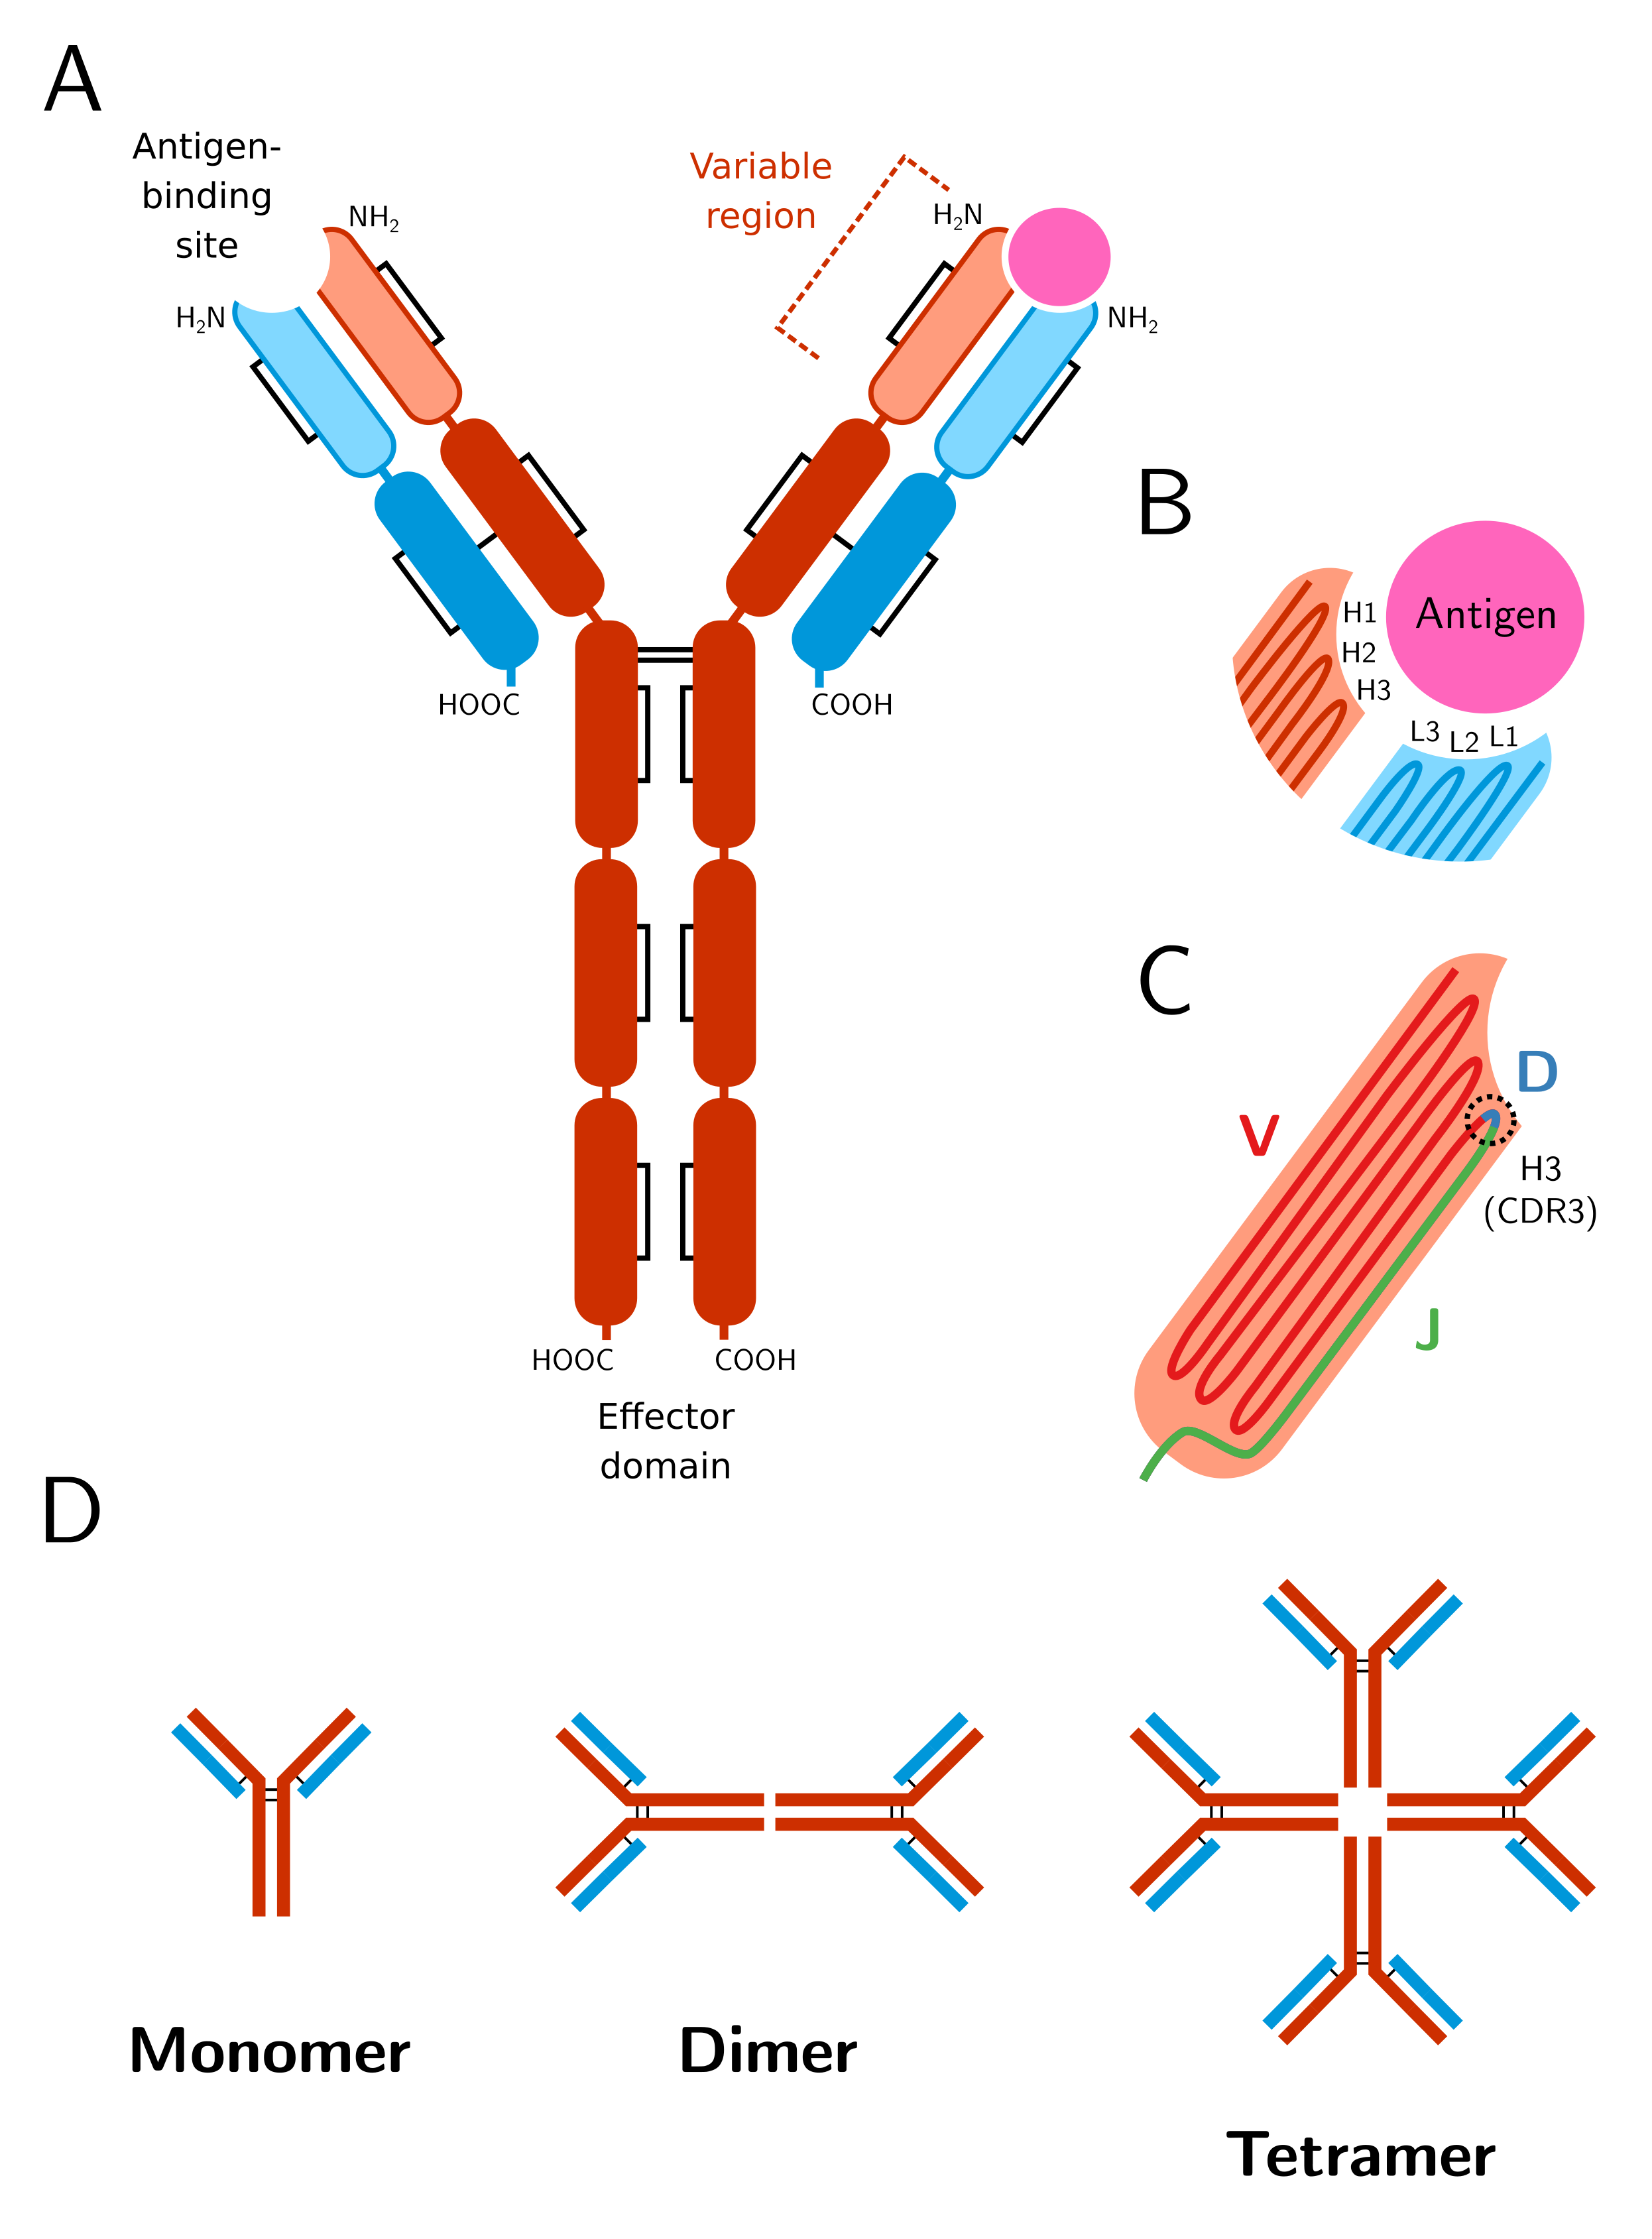
\includegraphics[width=0.9\textwidth]{_Figures/png_edited/antibody-structure}
\begin{subfigure}{0em}
\phantomsubcaption{}
\label{fig:intro-antibody-structure-schematic}
\end{subfigure}
\begin{subfigure}{0em}
\phantomsubcaption{}
\label{fig:intro-antibody-structure-loops}
\end{subfigure}
\begin{subfigure}{0em}
\phantomsubcaption{}
\label{fig:intro-antibody-structure-vdj}
\end{subfigure}
\begin{subfigure}{0em}
\phantomsubcaption{}
\label{fig:intro-antibody-structure-multimers}
\end{subfigure}
\caption[Antibody structure and function]{\textbf{Antibody structure and function:} (A) Schematic of a hingeless secreted antibody monomer, with heavy chains depicted in red, light chains in blue, and bound antigen in pink. Immunoglobulin fold domains are depicted as rounded rectangles, with variable-region domains shown with light shading and constant-region domains with dark. Black lines indicate disulfide bonds. (B) Schematic close-up of an immunoglobulin antigen-binding site, indicating the six loop regions (H1-3 and L1-3) making up the antigen-binding region. (C) Schematic close-up of the heavy-chain variable region, indicating the regions corresponding to the variable, diversity and joining gene segments from the unrecombined \igh{} locus. Note the chimeric nature of the third antigen-binding loop (H3, marked), which is formed by parts of all three gene segments. (D) In the context of antibodies, ``monomer'' refers to a single four-chain antibody protein, while ``dimer'', ``tetramer'' \etc refer to multiple antibodies linked together through covalent or noncovalent interactions.}
\label{fig:intro-antibody-structure}
\end{figure}
% TODO: Actual antibody crystal structure here?
% TODO: Discuss disulfide bonds in text
% TODO: Refer to VDJ schematic (1C) in next section

\subsection{Antibody sequence diversification and primary repertoire diversity}
\label{sec:intro_immunity_primary}

% TODO: Discuss allelic exclusion (Magadan)
% TODO: Discuss where primary and secondary diversification occur in fishes, and where B-cells reside (Mashoof)

The immune environment encountered by a vertebrate organism contains an enormous number of different potential pathogenic threats, each of which has its own antigenic signatures and many of which are capable of evolving much more rapidly than the vertebrate host \parencite{jack2015evolution}. In order for the adaptive immune system to cope with this huge diversity of different threats, it must be able to produce antibodies with a correspondingly large diversity of different antigen specificities. The greater the potential diversity of antibody sequences available to the adaptive immune system, the greater its capacity to respond effectively to novel immune threats. In reality, the mechanisms employed by the vertebrate adaptive immune system to diversify its antigen receptors enable an almost unlimited diversity of potential antibody sequences, with a correspondingly vast array of potential antigen specificities \parencite{mora2016quantifying}.

The mechanisms by which the adaptive immune system produces this diversity are dramatic, and rely on a highly unusual underlying gene structure \parencite{jung2006vdjr} and a very high level of cellular wastage \parencite{kogut2012bcells}. In the humoral immune system, antibody diversification takes place during B-cell development in the primary lymphopoietic organs (bone marrow in mammals, anterior kidney in teleosts \parencite{sunyer2013fishing}). Prior to this process, the native antibody loci in B-progenitor cells (and other cell types) is highly fragmented \parencite{jung2006vdjr}, with numerous fragmentary variable-region sequences present in series on the chromosome upstream of the constant-region exons. In the heavy chain locus, these variable-region gene segments can be divided into three categories:

\begin{itemize}
\item \textbf{Variable (\vh) segments} are the longest class of gene segment, at roughly \bp{300} in length. Each V-segment codes for the majority of the variable region of an antibody, including the entirety of the first three framework regions (FWR1-3) and the first two complementarity-determining regions (CDR1-2) as well as the 5' part of CDR3 \parencite{jung2006vdjr} (\Cref{fig:intro-antibody-structure-vdj}). They are therefore highly structured, and include several highly-conserved positions present in virtually all functional V-segments in nearly all species, including two conserved cysteine residues (which code for an intra-domain disulfide bond) and a conserved tryptophan residue following CDR1 \parencite{lefranc2003vnumbering}. Each V-segment is also associated with its own promoter sequence and 5'-UTR, as well as a 5'/C-terminal leader peptide between the translation start site and the start of the functional V-sequence.
\item \textbf{Diversity (\dh) segments} are the shortest class of segment, typically on the order of 10-\bp{20}, and are the least structured \parencite{ruiz1999humandj}. They form the middle part of CDR3 (\Cref{fig:intro-antibody-structure-vdj}) \parencite{schroeder2010immunoglobulins}.
\item \textbf{Joining (\jh) segments} are of intermediate length, typically 50-\bp{60} \parencite{ruiz1999humandj}. They form the 3'/C-terminal part of heavy chain CDR3 and the 5'/N-terminal part of FR4 (\Cref{fig:intro-antibody-structure-vdj}) \parencite{schroeder2010immunoglobulins}. Each J-segment is succeeded on the chromosome by a splice donor site \parencite{magadan2011medaka}, which is used to join the variable region of the antibody sequence to the constant region via RNA splicing following transcription of \igh{} mRNA (\Cref{fig:intro-vdjr-locus}iii). Like \vh segments, \jh segments can be identified from their conserved structure, particularly the conserved tryptophan residue marking the end of CDR3 \parencite{ruiz1999humandj}.
\end{itemize}

In the simplest ``translocon" configuration of the \igh{} locus, blocks of repeated \vh, \dh and \jh segments are present in series on the chromosome in contiguous V-, D- and J-regions (\Cref{fig:intro-vdjr-locus}i) \parencite{schroeder2010immunoglobulins,jung2006vdjr}. During B-cell development, a single \vh, \dh and \jh segment are selected, and the intervening genomic regions are permanently excised from the genome to produce a single contiguous VDJ sequence coding for the complete variable region of an antibody (\Cref{fig:intro-vdjr-locus}ii). The mechanism by which this excision occurs is called VDJ recombination, and relies on a specialised recombinase complex containing lymphocyte-specific recombination-activating genes 1 and 2 (\gene{RAG1} and \gene{RAG2}) \parencite{jung2006vdjr,schatz2011vdjr}. This complex recognises specialised recombination signal sequences (RSSs) flanking each variable gene segment, composed of highly conserved heptamer and nonamer sequences separated by a spacer sequence of conserved length (either 12 or \bp{23}, corresponding respectively to one or two turns of the DNA helix) \parencite{hesse1989rss} (\Cref{fig:intro-vdjr-consensus}). Each functional \vh segment is succeeded by a \bp{23}-spacer RSS in 5'-3' orientation, while each \jh segment is preceded by a \bp{23}-spacer RSS in 3'-5' orientation; each \dh segment, meanwhile, is flanked by \bp{12}-spacer RSSs in 5'-3' and 3'-5' orientation, respectively (\Cref{fig:intro-vdjr-rss}) \parencite{schatz2011vdjr}. 

In VDJ recombination, recombinase complexes bind two of these RSSs and associate with each other to bring the two corresponding gene segments into close proximity (\Cref{fig:intro-vdjr-mechanism}i-iii). A single-strand DNA nick is introduced between each RSS and its gene segment, and the exposed 3'-hydroxyl group of the break attacks the 5'-phosphate on the other strand to produce an asymmetric double-strand break, with the coding sequence terminating in a hairpin loop and the cleaved RSS in a blunt end \parencite{schroeder2010immunoglobulins,schatz2011vdjr} (\Cref{fig:intro-vdjr-mechanism}iv-v). These breaks are then resolved by the ubiquitous non-homologous end-joining machinery of the DNA damage response: the blunt ends of the cleaved RSSs can be directly ligated together, while for the coding sequences the hairpin loops must first be cleaved and the resulting 3'-overhangs resolved \parencite{schroeder2010immunoglobulins,schatz2011vdjr} (\Cref{fig:intro-vdjr-mechanism}vi-vii). The net result of this process is a contiguous V/D or D/J join in the coding sequence and a ligated DNA circle containing the excised RSSs and intervening sequence, which is subsequently degraded. Via unknown mechanisms \parencite{schatz2011vdjr}, the recombination machinery exhibits a strong preference for RSS sequences of different lengths (the so-called ``12/23 rule''), encouraging  D-J and V-D joins while largely preventing V-J joins. 

The simple joining of gene segments during VDJ recombination provides a basic combinatorial sequence diversity, with a number of possible sequences in the simplest case equal to the product of the numbers of \vh, \dh and \jh segments in the \igh{} gene locus. The number of potential \igh{} variable-region sequences in most species, however, is vastly higher than this: in humans, for example, there are roughly 8000 possible functional VDJ combinations \parencite{lefranc2001humanheavy}, but the number of different possible nucleotide sequences exceeds $10^{22}$ \parencite{elhanati2015model}. This huge difference arises from the inexactness with which the coding ends produced by the recombinase complex are joined following RSS excision (\Cref{fig:intro-vdjr-junctions}). Before the two gene segments brought together in VDJ recombination can be joined by NHEJ, the hairpin loops formed by the recombinase complex must be resolved by re-nicking the DNA \parencite{schroeder2010immunoglobulins,schatz2011vdjr}. This re-nicking process is not exact, and often occurs within the coding sequence, resulting in a palindromic 3'-overhang that can be filled in (resulting in palindromic \textit{P-insertions}) or trimmed (resulting in \textit{deletions}). The resulting blunt ends then serve as substrates for the lymphocyte-specific terminal dideoxy transferase enzyme (TdT), which adds a variable number of untemplated nucleotides (nonpalindromic \textit{N-insertions}) prior to sequence ligation \parencite{schroeder2010immunoglobulins,schatz2011vdjr}. As a result, the final recombined sequence is frequently not a clean ligation of the two original gene segments, but an inexact join involving multiple missing terminal positions and/or \textit{de novo} inserted sequence, a phenomenon collectively known as \textit{junctional diversity} (\Cref{fig:intro-vdjr-mechanism}vi-vii) \parencite{flaherty2012chapter}.

The three process contributing to junctional diversity (P insertion, N insertion, and deletion) together vastly increase the potential antibody sequence diversity available to a developing B-cell at the heavy-chain CDR3 region, which as a consequence is by far the most variable single region in determining antigen specificity \parencite{shirai1999h3}. This junctional diversity, however, comes at a substantial cost. The indel mutations introduced by VDJ recombination are not constrained to occur in multiples of three over both junctions, resulting in a high rate of recombinations in which the \vh and \jh segments are out of frame with each other; still more loci are rendered nonfunctional through the introduction of \textit{de novo} STOP codons. As the sequence changes introduced by VDJ recombination are irreversible, many developing B-cells are left with permanently disrupted \igh{} loci on both chromosomes, and are left with no recourse but programmed cell death. In addition, the huge and untemplated sequence diversity introduced in this way means that many B-cells whose \igh{} loci do successfully undergo VDJ recombination are left with BCRs that either cannot effectively bind any antigen or strongly bind self-antigen, resulting in useless antibodies in the first case and a dangerous risk of autoimmunity in the second; these B-cells are eliminated through a process of antigenic selection before \naive B-cells are permitted to exit the primary lymphopoietic organs, resulting in still more wastage as cells with nonfunctional or self-binding antigens undergo programmed cell death. Overall, as many as 90\% of developing B-cells may be eliminated by one or other of these processes before successfully exiting the primary lymphoid organs \parencite{kogut2012bcells}.  

% More details on primary selection in Kogut and its sources if needed

Taken together, the processes of VDJ recombination, junctional diversity and primary selection will produce a population of \naive B-cells with an extremely high diversity of heavy-chain ideotypes, with virtually every \naive B-cell expressing a unique variable-region sequence. Taken together, the resulting population of sequences represents the \textit{primary antibody heavy-chain repertoire} of the organism, and determines the range of different antigen sequences the humoral immune system of that organism can potentially respond to. The diversity of this primary repertoire depends on the native structure of the \igh{} locus in that species (which determines the number of segment choices available to the VDJ-recombination process), the distribution of possible numbers of insertions or deletions contributing to junctional diversity, and the stringency of the primary selection process.

\begin{figure}
\centering
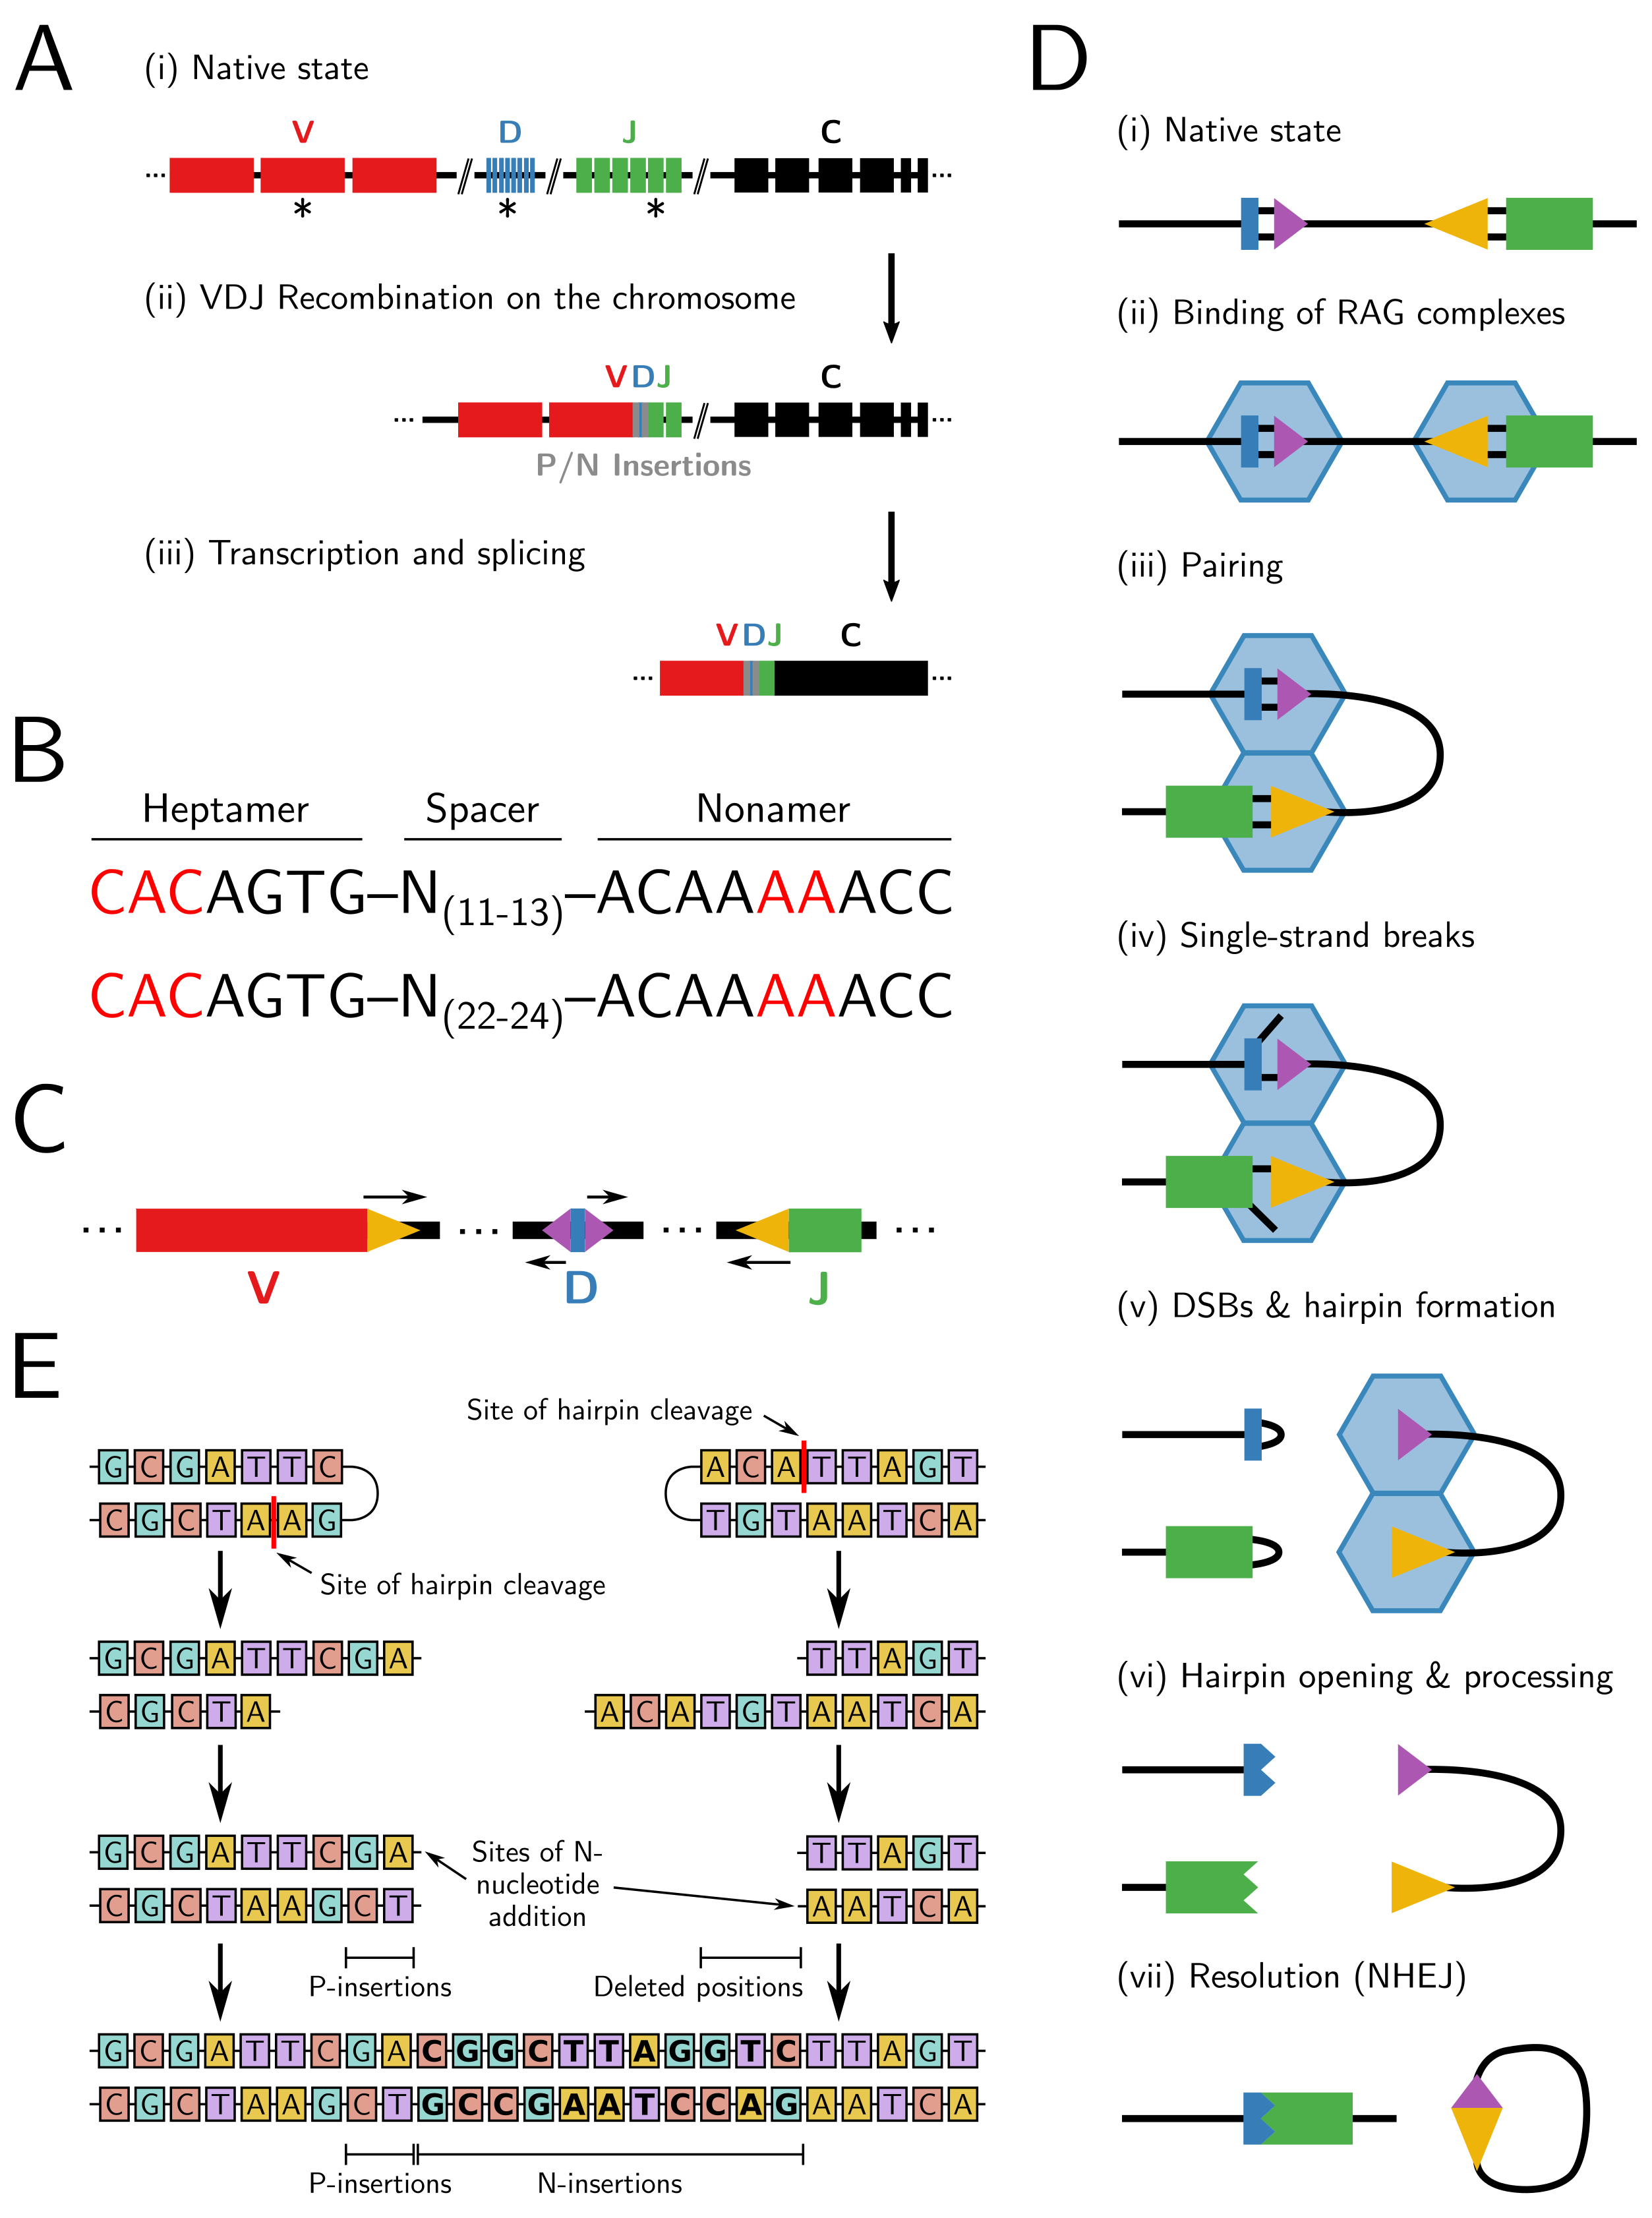
\includegraphics[width=0.95\textwidth]{_Figures/png_edited/primary-diversity}
\begin{subfigure}{0em}
\phantomsubcaption{}
\label{fig:intro-vdjr-locus}
\end{subfigure}
\begin{subfigure}{0em}
\phantomsubcaption{}
\label{fig:intro-vdjr-consensus}
\end{subfigure}
\begin{subfigure}{0em}
\phantomsubcaption{}
\label{fig:intro-vdjr-rss}
\end{subfigure}
\begin{subfigure}{0em}
\phantomsubcaption{}
\label{fig:intro-vdjr-mechanism}
\end{subfigure}
\begin{subfigure}{0em}
\phantomsubcaption{}
\label{fig:intro-vdjr-junctions}
\end{subfigure}
\caption[Primary sequence diversification in antibodies]{\textbf{Primary sequence diversification in antibodies:} (A) Schematic of antibody sequence formation at the locus level. Black asterisks indicate the segments to be recombined. (B) Consensus sequence of short (above) and long (below) RSSs in jawed vertebrates. Nucleotides marked in red are the most strongly conserved and most required for efficient recombination \parencite{hesse1989rss}. (C) Schematic of position and orientation of long (orange) and short (purple) RSSs relative to variable-region gene segments. (D) Schematic of recombination mechanism for a D/J segment pair, illustrating hairpin formation and imprecise end-joining of coding sequences; adapted from \parencite{schatz2011vdjr}, Figure 2. (E) Example of the inexact hairpin resolution mechanisms leading to junctional diversity in (D-vi); adapted from \parencite{flaherty2012chapter}, Figure 10-5.
} 
\label{fig:intro-vdjr}
\end{figure}


%VDJ recombination in the \textit{IGH} locus is highly structured, and occurs in a specific order. First, a D and a J segment are selected and recombined to produce a DJ sequence. Then, a V region is selected and recombined with the DJ to produce a continuous VDJ sequence constituting the variable region of the heavy chain. The complete protein sequence is produced during later transcriptional splicing, which joins this variable-region sequence to downstream constant-region exons to produce a mature \textit{IGH} mRNA. This strict ordering of V/D/J segments, which obtains in the vast majority of recombined sequences observed, is produced through the combination of a variety of regulatory mechanisms. The most basic of these is the structure of the RSSs, which comprise a conserved heptamer and nonamer sequence separated by a relatively unconserved spacer region of either 12 or 23bp \parencite{jung2006vdjr}, corresponding to either one or two turns of the DNA helix. V and J segments in the IGH locus are flanked by RSSs with 23bp spacer regions, while those flanking D-regions have 12bp spacers %citation needed
%As the RAG recombinase specifically recognises pairs of RSSs with dissimilar spacer lengths (a restriction known as the 12/23 or one-turn/two-turn rule), direct V-to-J recombination events are excluded \parencite{jung2006vdjr}. % Better citation if possible.
%
%Complete VDJ recombination places the V-region promoter in close proximity to a highly-conserved enhancer element (known as iE$\mu$) lying between the last J segment and the first constant-region exon \parencite{jung2006vdjr}; this enhancer is important for strong expression of the mature IGH mRNA from the pre-B-cell stage onwards. 

\subsection{\igh{} locus structure in teleost fishes}
\label{sec:intro_teleost_loci}

\Cref{sec:intro_immunity_primary} describes the process of \igh{} locus maturation in terms of an idealised translocon locus with a simple V-D-J-C structure (\Cref{fig:intro-vdjr-locus}). In some species, including humans and mice, \igh{} loci roughly correspond to this simplified structure, albeit with a much larger number of gene segments; however, in many species, including all teleosts, this idealised structure is a significant oversimplification of the actual layout of their \igh{} loci. Due to their repetitiveness and complex structure, comprehensive assembly of \igh{} loci is often difficult, and full elucidation of their structure often requires a focused characterisation effort. % Citation needed
Nevertheless, a number of teleost loci have been characterised to date, including several species (e.g. three-spined stickleback and medaka) closely related to the African turquoise killifish.

Among teleost fishes, the simplest \igh{} locus structures known to date are exhibited by species such as zebrafish, grasscarp, and fugu (\Cref{fig:intro-teleost-loci-simple}) \parencite{fillatreau2013astonishing}. In these species, the \igh{} locus adopts a V-D-J-\cz{}-D-J-\cm{}-\cd{} structure, with a single shared V-region followed by D- and J-regions specific to the \igh{Z} and \igh{M/D} constant regions, respectively. The rainbow trout locus has a similar organisation, but with two additional V-segments following the \igh{Z} region \parencite{hansen2005trout}. During VDJ recombination in these loci, the choice of variable gene segments also determines the choice of constant region: if a pair of \dh and \jh segments upstream of the \igh{Z} constant region is selected, the cell will express \igh{Z}, while if the segments chosen are downstream of \igh{Z}, that constant region will be excised during VDJ recombination and \igh{M} and/or \igh{D} will be used instead. As a result, VDJ recombination in these species determines both the ideotype of a developing B-cell and its isotype \parencite{fillatreau2013astonishing}.

While some teleost species possess such relatively simple \igh{} loci, many species exhibit much more complicated, and often much larger, locus structures. In many species, multiple distinct subloci (comprising V-, D- and J-regions and least one constant region) are present in tandem on the chromosome, often with distinct combinations of variable gene segments and constant regions (\Cref{fig:intro-teleost-loci-complex}); in a few cases, such as medaka and Atlantic salmon, one or more of these subloci is in inverted orientation relative to the rest of the locus. In some species, such as Atlantic salmon, whole-genome duplication has led to the existence of multiple distinct \igh{} loci on different chromosomes, each of which has its own complement of subloci, gene segments, and constant regions \parencite{yasuike2010salmon}. In this milieu, pseudogenisation of gene segments or constant-region exons is common, resulting in loci with large numbers of pseudogenised V-segments and constant regions.

The diversity in locus size and organisation among teleost fishes is likely to have important consequences for humoral adaptive immunity in these species. The native locus constitutes the raw substrate for the VDJ recombination process, and the number of different \vh, \dh and \jh gene segments available for recombination defines the baseline sequence diversity of antibodies in that species. It is not clear to what extend VDJ recombination can take place across different subloci in the large tandem loci described in \Cref{fig:intro-teleost-loci-complex}; if recombination between subloci is restricted, this will also have important effects on the kinetics of VDJ recombination in a species. The division of an \igh{} locus into tandem subloci may also have effects on the statistics of B-cell maturation, with more subloci conceivably presenting the opportunity for a greater number of recombination attempts before the \igh{} loci of a developing B-cell are exhausted and so reducing the rate at which cells fail to mature successfully; however, to my knowledge little or nothing is known about the effects of locus structure on B-cell developmental processes at present. Finally, variations in the constant regions present in different species are likely to have very important effects on humoral immunity; most fundamentally, whereas \igh{Z/T} appears to be specialised for mucosal adaptive immunity in those teleost species that possess it \parencite{zhang2010igtgut,fillatreau2013astonishing,xu2013igtskin}, it is not known how mucosal immune responses manifest in species lacking this isotype. Given all these important (and potentially-important) effects of \igh{} locus structure on humoral adaptive immunity, characterising the sequence and organisation of this locus is an essential step in understanding the adaptive immune system of any vertebrate species.

% TODO: Read up on allelic exclusion in teleosts in Magadan 2015

\begin{figure}
\centering
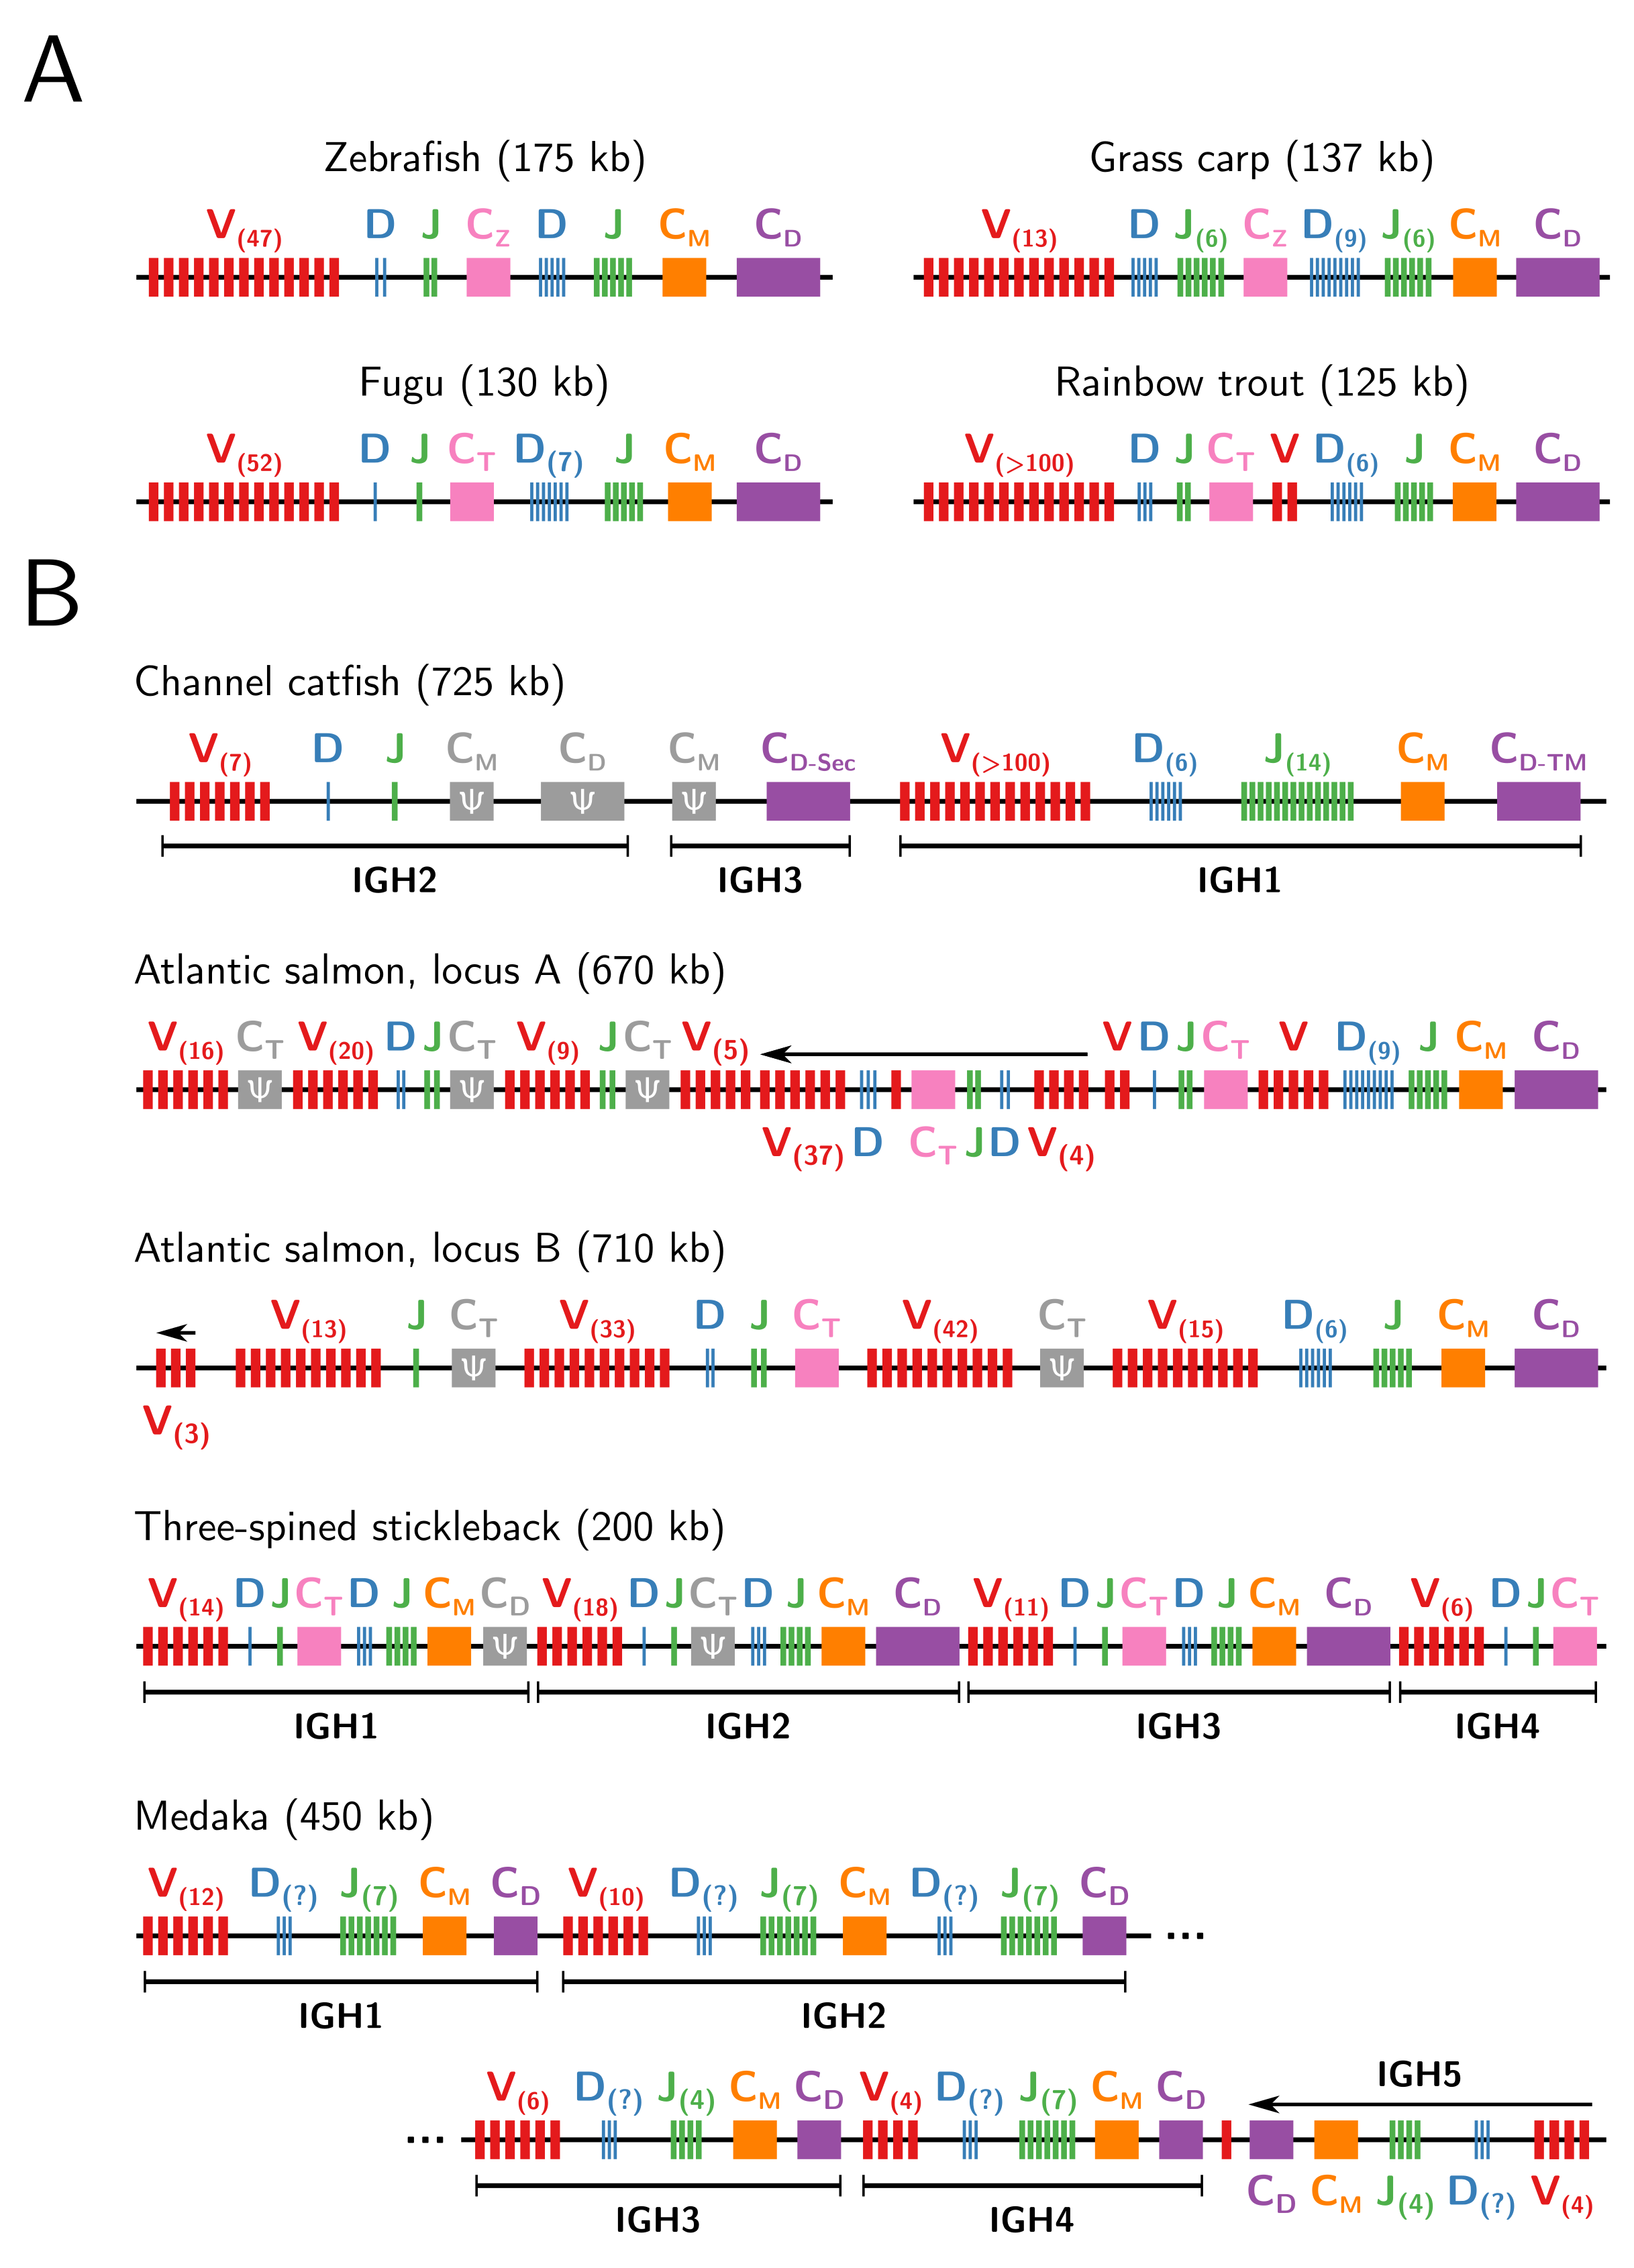
\includegraphics[width=0.85\textwidth]{_Figures/png_edited/teleost-loci}
\begin{subfigure}{0em}
\phantomsubcaption{}
\label{fig:intro-teleost-loci-simple}
\end{subfigure}
\begin{subfigure}{0em}
\phantomsubcaption{}
\label{fig:intro-teleost-loci-complex}
\end{subfigure}
\caption[\igh{} locus structure in teleost fishes]{\textbf{\igh{} locus structure in teleost fishes:} Simplified schematics of \igh{} loci from nine teleost species. (A) In the simplest teleost \igh{} loci, single \igh{Z} and \igh{M/D} constant regions share a common V-region, but are preceded by separate D/J regions. In rainbow trout, a small number of V-segments also separate \igh{Z} from the pre-\igh{M} D-region. (B) In many teleosts, the \igh{} loci are much larger and more complex, with repeated tandem subloci (labelled regions), pseudogenised constant regions (grey, $\psi$), inverted segments (leftward arrows), and other deviations from the classic locus organisation. Loci are not to scale; blocks of more than five segments are condensed and labelled with their segment number, as are some smaller segment blocks for clarity. Adapted from \parencite{fillatreau2013astonishing}, Figure 2 and \parencite{bengten2015fishantibodies}, Figure 4, with additional information from \parencite{magadan2011medaka,bao2010stickleback,gambondeza2011stickleback,yasuike2010salmon,xiao2010grasscarp}.
The number of D-regions in the medaka locus is not provided in the sources.}
\label{fig:intro-teleost-loci}
\end{figure}

\subsection{Affinity maturation and secondary repertoire diversity}
\label{sec:intro_affinity_maturation}

Following VDJ recombination and primary selection, developed \naive B-cells emerge from the primary lymphoid organs and circulate in the periphery. At some point, a subset of these \naive cells will make contact with their cognate antigen. If this contact occurs in the correct signalling context (in particular, in the presence of T-cell help), % TODO: Explain this better, add a citation
the B-cell becomes activated and begins to proliferate. During this clonal expansion process, the B-cell's antibody genes undergo a very high rate of somatic mutation (known as \textit{somatic hypermutation} or SHM), with mutations focused in the complementarity-determining regions coding for the antigen-binding loops of the variable region; in mammals, the rate can be as high as $10^{-3}$ per nucleotide per cell division \parencite{noia2007shm}. This SHM process is orchestrated by the activation-induced cytidine deaminase enzyme (AID), which preferentially targets particular hotspot motifs (canonically  RGYW/WRCY and WA/TW) and deaminates cytidine residues to uracil, which can either be corrected to thymine on DNA replication (resulting in a C-to-T transition mutation) or removed via base-excision repair (resulting in a variety of other mutations) \parencite{magor2015affinity}. As a result, the original antibody sequence of the ancestral \naive cell is diversified into a cluster of related sequences, with widely varying affinity for the cognate antigen.

In order for the combination of clonal expansion and somatic hypermutation to improve the adaptive immune system's ability to respond to the stimulating antigen, the resulting clone needs to undergo a selection process, to identify and advantage cells expressing antibodies with improved antigen affinity. This selection is effected through a competitive process in which clonally-expanded B-cells attempt to bind cognate antigen trapped on the surface of helper cells: those cells which successfully bind antigen receive growth and differentiation signals, while those which do not undergo programmed cell death. In mammals, this process takes place primarily in histologically-distinct germinal centres within specialised secondary lymphoid organs such as the spleen, in which B-cells that have encountered antigen first undergo clonal expansion and SHM, then compete for antigen on the surface of follicular dendritic cells. In teleosts, which lack specialised, histologically-differentiated germinal centres, B-cell proliferation takes place near clusters of melanomacrophages surrounded by reticular cells, both of which have been attributed an antigen-trapping and -presentation role analogous to that performed by FDCs in mammals \parencite{magor2015affinity}. % TODO: Citation for germinal centres

While clonal expansion, somatic hypermutation and clonal selection, collectively known as \textit{affinity maturation}, are present in both mammals and teleosts, the increase in antibody affinity resulting from this process in teleosts is far weaker than in mammals (e.g. 3-to-10-fold in rainbow trout, compared to as much as 1000-fold in mammals \parencite{magor2015affinity}). Since SHM appears to be fully functional in those fish so far investigated (albeit with a greater bias towards C-to-T transitions over other mutations) \parencite{magor2015affinity}, this difference seems likely to arise from differences in clonal selection dynamics between teleosts and mammals. The reasons for such a difference are still not entirely clear, but may involve histological differences in where and how affinity maturation takes place in these taxa. In mammalian germinal centres, the ratio between expanded B-cells and FDCs is such that the amount of presenting antigen is limiting, forcing competition for antigen among B-cells and favouring those cells which can bind antigen most strongly \parencite{magor2015affinity}. In teleosts, conversely, proliferating B-cells are far outnumbered by antigen-trapping melanomacrophages and reticular cells, resulting in an oversupply of antigen relative to B-cell demand; this antigen surplus may result in faster overall proliferation, but at the cost of much weaker selection for high-affinity antibodies \parencite{magor2015affinity}.

Following affinity maturation, activated B-cells undergo differentiation into memory cells (which persist in the bloodstream for long periods and provide secondary immune memory) and plasmablasts/plasma cells (which secrete large amounts of antigen to mount a powerful immune response). Affinity-matured cells can also re-enter germinal centres (or their less-developed teleost equivalents) to undergo additional rounds of proliferation, hypermutation and selection; memory cells can also undergo further rounds of affinity maturation, resulting in even larger and more diverse clones and still-higher levels of antigenic affinity. In tetrapods, class switching between different constant-region isotypes also occurs as part of affinity maturation, and is also orchestrated by AID; however, this process is absent in teleosts. % TODO: Citation(s) needed

The combination of the primary (\naive) repertoire described in \Cref{sec:intro_immunity_primary} with the clonal expansions and additional sequence diversity arising from affinity maturation constitutes the \textit{secondary heavy-chain antibody repertoire} of the organism (\Cref{fig:intro-bcell-repertoires}). This is the repertoire actually encountered by incoming pathogens and available to relatively direct experimental interrogation. The structure and diversity of this secondary repertoire depends on the makeup of the primary repertoire, the degree of clonal expansion and hypermutation during affinity maturation, the strength of clonal selection, and the relative abundance of different B-cell subtypes. Inferring the composition of the primary repertoire from that of the secondary is therefore non-trivial, and requires an attempt to distinguish sequences arising from \naive versus activated B-cells or infer the former from the latter; once obtained, the \naive sequences can be used to infer the parameters of the generative process \parencite{elhanati2015model}.

\begin{figure}
\centering
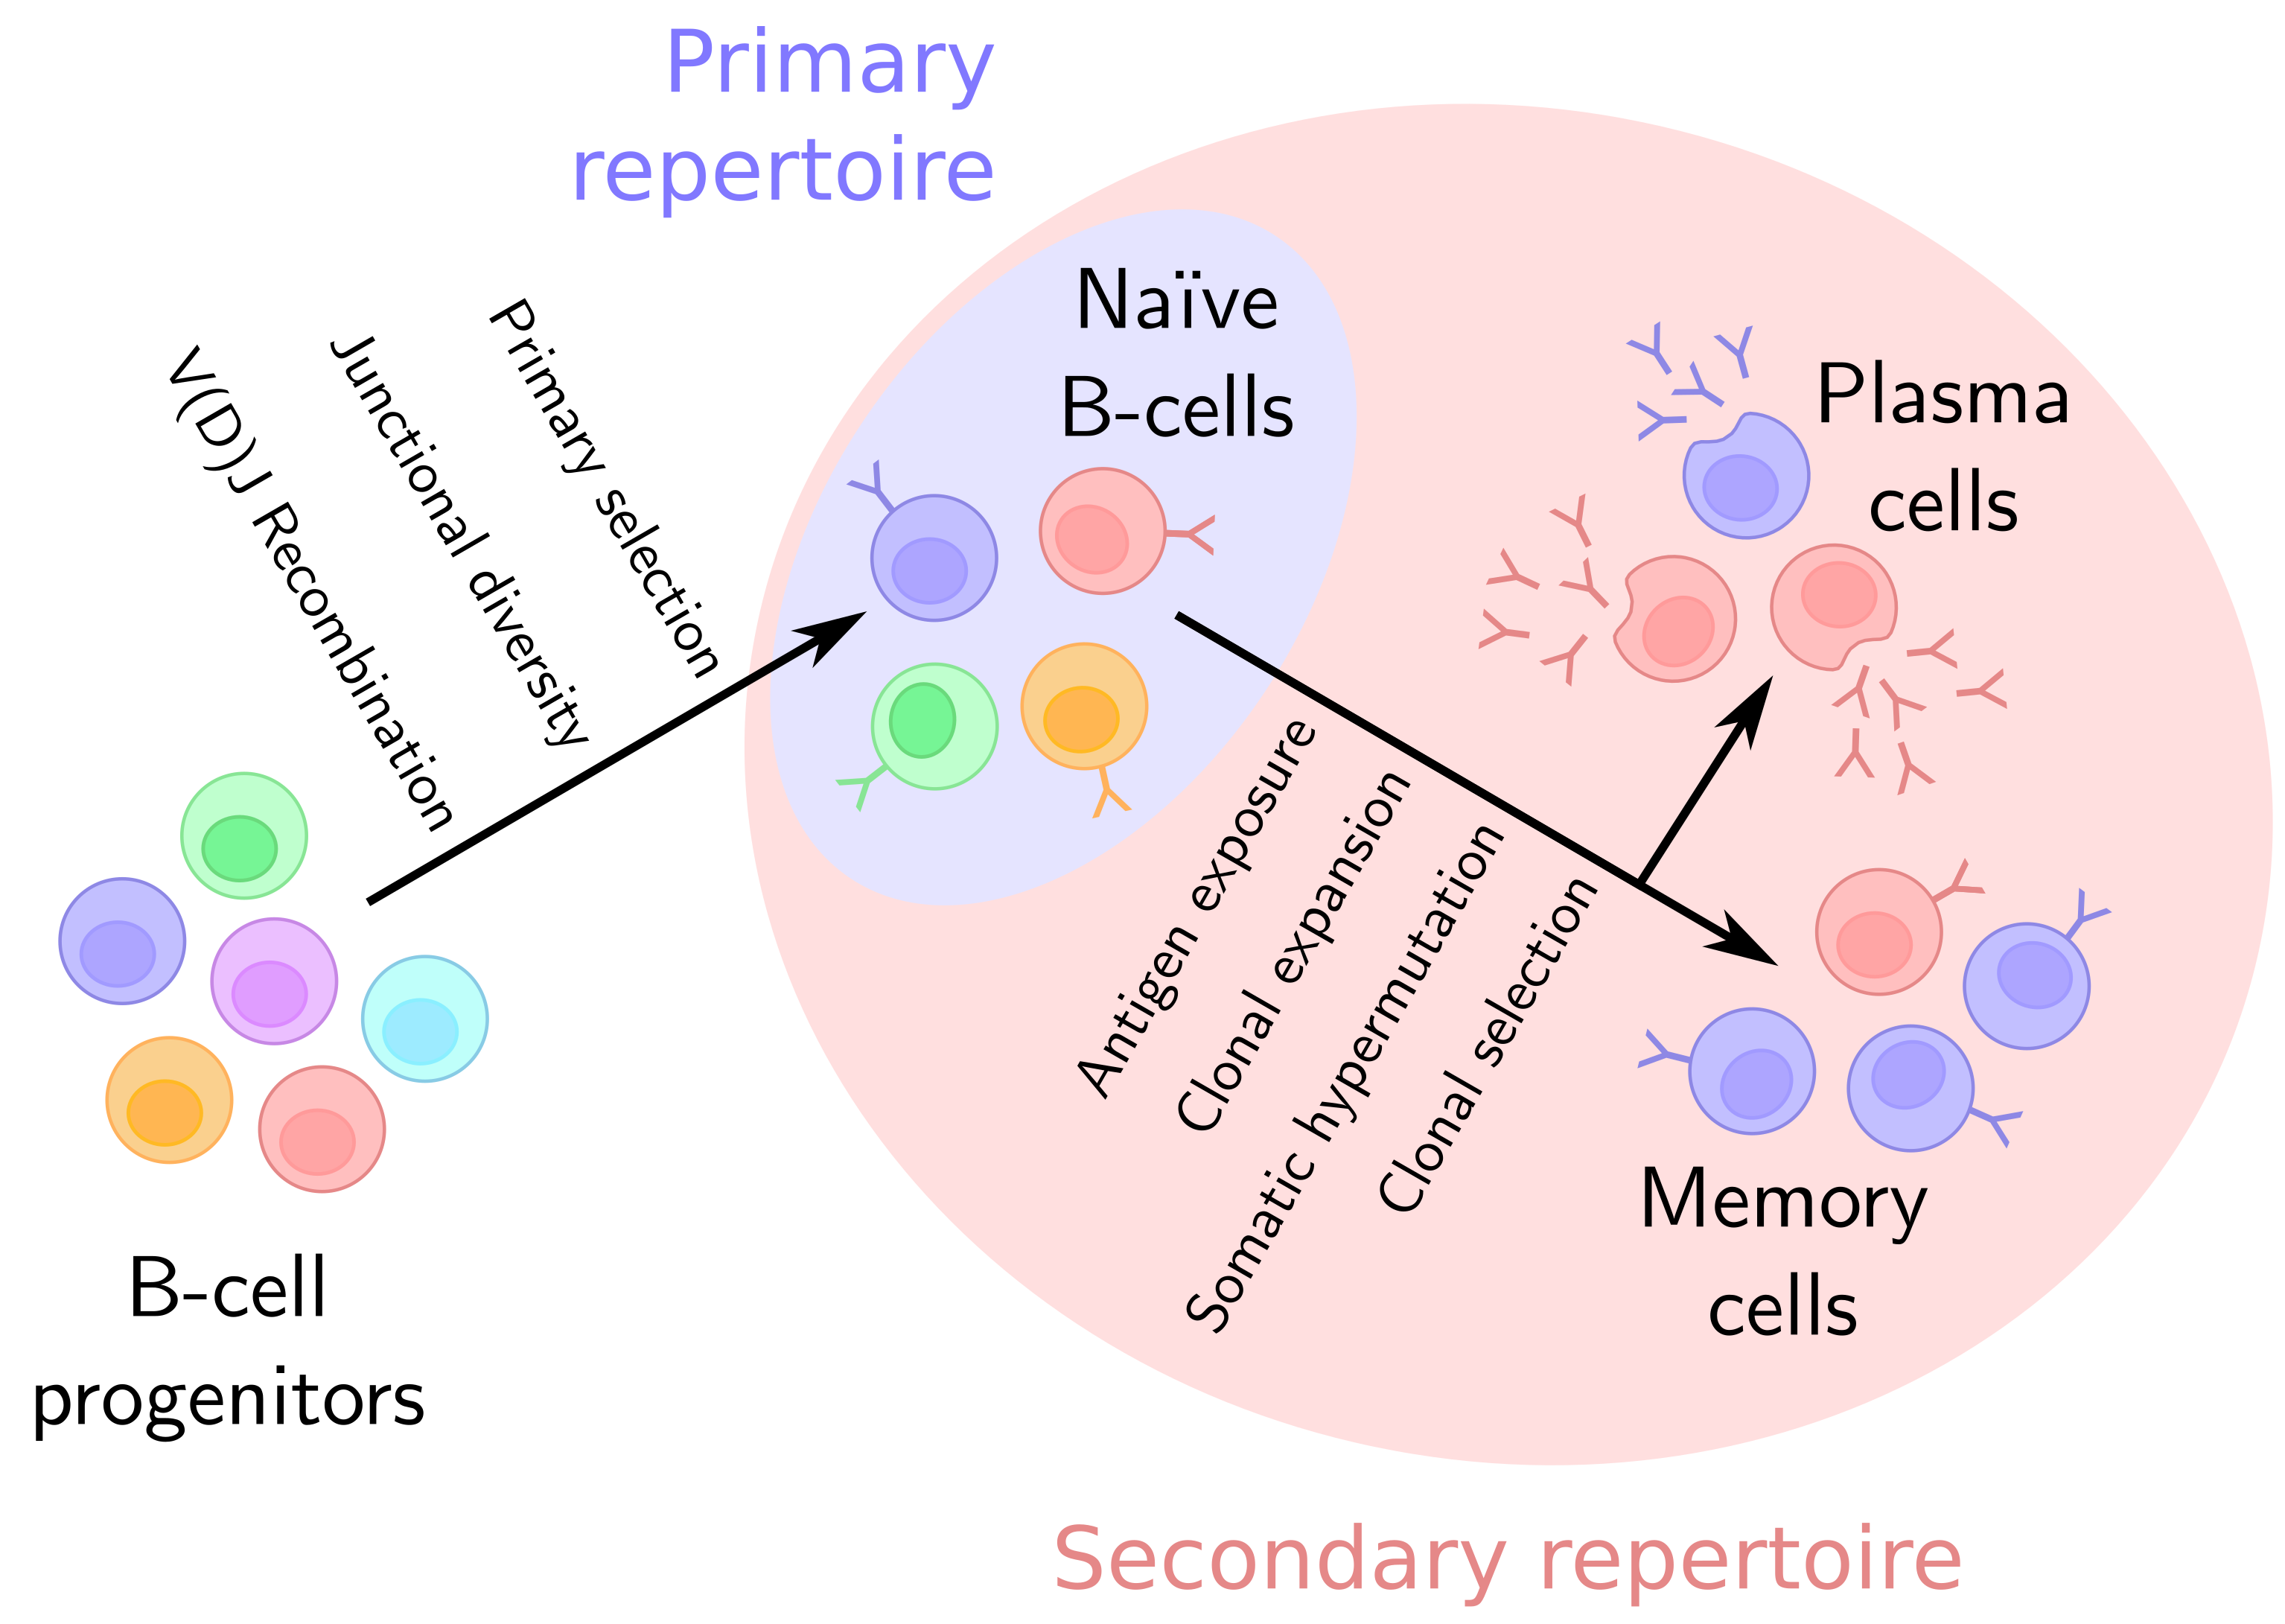
\includegraphics[width=0.9\textwidth]{_Figures/png_edited/bcell-repertoire-primary-secondary}
\caption{\textbf{Primary and secondary antibody repertoires:} Schematic of processes giving rise to the primary (\naive) and secondary (total) B-cell repertoires in the vertebrate immune system. Cell colours indicate clonal membership, with a loss of clonal diversity during primary development (left) and affinity maturation (right). Primary B-cell development (left) takes place in primary lymphoid organs (bone marrow in mammals, anterior kidney in teleosts), while affinity maturation (right) takes place in germinal centres (in mammals) or proto-germinal clusters (in teleosts) in secondary lymphoid organs such as the gut-associated lymphoid tissue (GALT) or spleen.}
\label{fig:intro-bcell-repertoires}
\end{figure}

\section{Humoral adaptive immunosenescence in vertebrates}
\label{sec:intro_immunosenescence}

The immune system of aged vertebrates has long been known to undergo a severe and systemic decline in functionality with age \parencite{segre1977immunosenescence}. As a result of this decline, older individuals exhibit increased susceptibility to a wide range of bacterial, viral, and fungal infectious diseases, as well as higher rates of complications and mortality from those infections when they occur \parencite{sambhara2009vaccination}. In addition, the effectiveness of vaccination against these infections often declines dramatically with age, with older individuals often receiving half or less of the immune protection from vaccination exhibited by younger recipients \parencite{sambhara2009vaccination}. Similar declines in immune functionality with age are also observed in other model organisms, and have been especially well-studied in mice, which share many details of their immune system with humans while being substantially easier to study in depth. While many different parts of the immune system are implicated in this immunosenescent phenotype \parencite{kogut2012bcells}, the decline in the humoral adaptive immune system has emerged as one particularly important contributor \parencite{ademokun2010ageing}.

The changes in the humoral immune system underlying its impaired functionality in old age begin at the level of B-cell development. In mice, the population of haematopoietic stem cells (HSCs) resident in the bone marrow increases in number but exhibits a decreased propensity to regenerate the pool of developing B-cells \parencite{ademokun2010ageing,kogut2012bcells}; factors contributing to this change include a deteriorating bone marrow niche, changes in blood-borne factors affecting HSC differentiation, and the well-known of older mammalian HSCs towards myeloid (rather than lymphoid) cell lineages \parencite{kogut2012bcells,dunnwalters2010bcellageing}. As a result of this change in HSC behaviour, the number of new B-cell progenitor and precursor cells in the bone marrow declines with age in mice; furthermore, these precursors exhibit decreased proliferation capacity, reduced rates of VDJ recombination and an increased rate of apoptosis \parencite{montecino2013immunosenescence,kogut2012bcells,labrie2004bone}. The rate of B-cell output from the bone marrow therefore declines significantly in aged mice compared to young adults, falling as low as 10\% of its level in young mice \parencite{kogut2012bcells}. As these \naive cells also have a shorter lifespan than antigen-experienced memory- and long-lived-plasma-cell populations, the net result of this decline in output from the bone marrow is a decrease in the number of \naive cells in the periphery and a progressive increase in the relative prevalence of antigen-experienced memory and plasma cells \parencite{mehr2011reversing,kogut2012bcells}; the pool of circulating immunoglobulins, meanwhile, becomes progressively dominated by hypermutated antibodies specific to previously-encountered antigens \parencite{kogut2012bcells}. As these \naive cells are essential for responding to novel or mutated immune threats not previously encountered by the immune system, this change is thought to lead to a progressive reduction in the capacity of the humoral immune system to respond effectively to novel threats \parencite{kogut2012bcells}.

Despite the decline in new \naive B-cells produced by the bone marrow, the total number of B-cells in aged mice does not appear to change significantly, reflecting an increase in the absolute number, as well as the relative prevalence, of antigen-experienced B-cell subpopulations. In humans, conversely, the absolute number of total B-cells appears to decline with age \parencite{ademokun2010ageing,montecino2013immunosenescence,aberle2013mechanistic}, with most B-cell subsets showing a significant decline in absolute abundance \parencite{frasca2011age}. Sources differ as to the age-related changes in relative abundance of different B-cell subtypes in humans, with some reporting an increase in the relative prevalence of \naive cells and decrease in that of memory cells\parencite{frasca2011age,blomberg2013age} and others reporting a more mouse-like shift in favour of the memory compartment \parencite{ademokun2010ageing}. These differences may arise from differences in the methods and cell markers used to quantify abundance of different B-cell populations \parencite{ademokun2010ageing}, genuine differences between populations, or the limitations of peripheral blood as a method of sampling the whole-body B-cell population of an individual \parencite{siegrist2009extremes}.

Whatever changes in cellular composition occur in ageing humans, it is clear that both humans and mice undergo a severe age-related decline in B-cell functionality. In humans, the best-understood aspect of this decline is a deterioration in the responsiveness of older patients to vaccination. Older humans frequently exhibit a substantially smaller \parencite{sambhara2009vaccination} and slower \parencite{kogut2012bcells} increase in the titre of antigen-specific serum antibodies in response to vaccination \parencite{sasaki2011limited,aberle2013mechanistic,ademokun2010ageing}, with defects in humoral response observed to vaccines for diseases as diverse as influenza, hepititis A and B, tetanus, diphtheria, pneumococcus and tick-borne encephalitis \parencite{dunnwalters2010bcellageing}. At least in the case of influenza, this decline in specific antibody production is primarily due to a decrease in the number of plasmablasts activated in response to vaccination \parencite{montecino2013immunosenescence,aberle2013mechanistic,sasaki2011limited}.

In addition to being less abundant, the antibodies produced by elderly humans in response to vaccination also appear to be of lower quality: anti-influenza antibodies produced by older human individuals demonstrate reduced ability to effectively neutralise viral haemagglutinin \parencite{kogut2012bcells,sasaki2011limited}, while IGHM antibodies produced by elderly subjects in response to pneumococcal polysaccharide vaccine demonstrate reduced opsonisation ability \parencite{kogut2012bcells}. While basal serum antibody titres actually increase rather than decrease with age in humans and mice \parencite{frasca2009ageing}, suggesting that antibody production \textit{per se} is not impaired with age, these antibodies also decline in quality \parencite{montecino2013immunosenescence}, with measurable increases in the rate of polyspecific and self-reactive antibodies produced in older individuals \parencite{kogut2012bcells}. This decline in baseline antibody quality in older individuals suggests a breakdown in primary B-cell selection in the bone marrow, enabling a greater number B-cells with low-specificity or self-reactive antibody sequences to emerge into the periphery \parencite{ademokun2010ageing}.

Various aspects of affinity maturation are also impaired in aged mammalian B-cells. While memory-cell clones established early in life often persist into old age, \naive B-cells in aged humans demonstrate a severely reduced ability to give rise to new antigen-specific memory B-cells following antigenic stimulation, impairing the establishment of functional immune memory for novel threats \parencite{aberle2013mechanistic}. B-cells from older humans and mice also exhibit impaired class-switch recombination capacity, possibly as a result of decreased AID expression \parencite{montecino2013immunosenescence,blomberg2013age,frasca2011age}, impairing the generation of antibodies with the same specificity but different effector functions. The decreased ability of older individuals to produce high-affinity antigen-specific antibodies \parencite{frasca2011age} also suggests a defect in affinity maturation, though this could also be attributable to the known ageing-related defects in the T-helper and follicular dendritic cells involved in secondary B-cell selection \parencite{montecino2013immunosenescence,aberle2013mechanistic,ademokun2010ageing} rather than changes in the B-cells themselves. Conversely, the effect of ageing on the somatic hypermutation process remains controversial \parencite{henry2019influenza,howard2006quality,ademokun2010ageing,frasca2009ageing}, with different groups reporting an increase, a decrease, or no change in the rate and level of SHM accumulation of different B-cell subtypes with age. 

The various cellular and population-level changes that occur in the humoral immune system with age naturally have important effects on the antibody repertoires of ageing individuals. Aged humans \parencite{siegrist2009extremes} and mice \parencite{dunnwalters2010bcellageing} exhibit increased rates of non-malignant clonal expansions in the memory-cell compartment, which when combined with the apparent maintenance or decline in total B-cell number would lead to a reduction in overall diversity \parencite{dunnwalters2010bcellageing}. Similarly, early techniques that investigated the repertoire by investigating the distribution of CDR3 lengths (CDR3 spetratyping) indicated that older humans frequently exhibit more distorted distributions dominated by CDR3 regions of a particular length, indicative of clonal expansion, and found that older individuals with more distorted spectratypes exhibited greater frailty and worse health and lifespan outcomes than those with more young-like spectratypes \parencite{gibson2009spectratyping}. On the basis of these and similar findings, the antibody repertoire has long been thought to decline in diversity in older individuals, impairing the adaptability of the ageing adaptive immune system.

More recently, the development of specialised high-throughput-sequencing-based techniques for interrogating antibody repertoires (\Igseq, or \igseq \parencite{weinstein2009igseq}) has enabled a few studies to investigate the ageing of these repertoires in greater detail. These studies, primarily on human peripheral blood, have confirmed many observations made using older lower-throughput methods: a reduced number of clonal lineages in older repertoires reflects decreased \naive-cell output from the bone marrow) \parencite{jiang2013vaccine}, while an increase in mean CDR3 length \parencite{wang2014ageing} and the average rate of premature STOP codons \parencite{debourcy2017ageing} in older repertoires similarly support the finding that primary and clonal selection are impaired with age. 
An increase in clonal expansion in older individuals is also observed: 
an \textit{oligoclonal} phenotype, in which one or a few large clones dominate the repertoire, is often seen in peripheral blood from elderly humans but very rarely in the young \parencite{wang2014ageing,debourcy2017ageing}. These expanded clones are persistent before and after vaccination \parencite{debourcy2017ageing} and even across multiple years \parencite{wang2014ageing}; in contrast, large clones observed in young human blood repertoires are typically transient responses to recent antigen challenge \parencite{wang2014ageing}.

The reduction in clonal richness and increase in clonal expansions seen in older individuals contribute to an overall reduction in the estimated number of unique sequences present in the peripheral repertoire \parencite{debourcy2017ageing}, a change observed for both \naive and mutated sequences and exacerbated by a significant reduction in within-clone sequence diversity in at least some elderly individuals \parencite{debourcy2017ageing}. The same study also found a drop in the percentage of unique sequences identified as coming from \naive B-cells, suggesting a mouse-like shift in repertoire prevalence towards antigen-experienced cell types \parencite{debourcy2017ageing}. However, while the alpha (within-individual) sequence diversity of the human peripheral repertoire appears to decline with age, the beta (between-individual) diversity of the repertoire actually increases, with repertoires from older individuals differing more from one another than those of young individuals \parencite{debourcy2017ageing}. Elderly repertoires also showed decreased flexibility in response to immune challenge, with repertoires taken from the same individual pre- and post-vaccination being significantly more similar in elderly than in young samples \parencite{debourcy2017ageing}, perhaps as a result of longer and more individualised histories of antigen exposure. Taken together, these findings suggest a pattern in which human peripheral antibody repertoires progressively lose diversity of the course of the human lifespan, while also becoming increasingly individualised and distinct.

In conclusion, there is strong evidence for a variety of developmental and physiological changes in the B-cell immune system with age in both mice and humans, giving rise to a severe decline in overall functional performance and immune protection. Many of these changes affect the composition of the antibody repertoire, with a reduction in clonal and sequence diversity and an increase in between-individual variability with age in human blood. However, despite this abundance of data, there remain some serious limitations in our knowledge of the ageing antibody repertoire.  From an evolutionary and comparative perspective, almost nothing is known about adaptive immunosenescence in species other than humans and mice; while several \igseq studies have been performed on teleost fish \parencite{weinstein2009igseq,jiang2011determinism,krasnov2017igseq,lund2019salmon,fu2018fugu}, for example, none to my knowledge have investigated B-cell immunosenescence in this taxon. Many of the findings reported above are specific to IGHG or IGHA antibodies in mice and humans \parencite{kogut2012bcells}, and may not generalise to species lacking these isotypes. Even in humans, the majority of immunosenescence studies, including virtually all repertoire studies, are limited to peripheral blood, and therefore primarily sample the minority of B-cells in transition between tissues; the majority of B-cells, which are resident in some immune organ or tissue, are systematically underrepresented in these samples \parencite{siegrist2009extremes,tabibiankeissar2016ageing}. Relatively little is therefore known about how the ageing of the B-cell repertoire differs between organs; the only paper I know of which investigated changes in antibody-repertoire diversity with age in biopsies from multiple human tissues failed to find any significant changes in alpha diversity, except for a significant \textit{increase} in repertoire sequence entropy in old spleen \parencite{tabibiankeissar2016ageing}. No published paper I know of has yet to investigate the ageing of the antibody repertoire at mucosal surfaces, where secreted antibodies play a particularly important role in regulating microbiotal communities and defending the body from pathogenic invasion.

In addition to this lack of spatial resolution in our knowledge of antibody repertoire ageing, there is a serious lack of temporal resolution; most studies of antibody repertoire ageing simply compare a ``young'' group (say 20-30 years of age) with one or two ``old'' groups (say $\geq70$ years of age), with little or no information about the intervening progression of any observed phenotypes \parencite{debourcy2017ageing,tabibiankeissar2016ageing}. The effect of known lifespan-increasing interventions on immune repertoire ageing also remains largely unstudied. Due to their very long lifespans and restrictions on experimental manipulation, humans are unsuitable subjects for these sorts of experiments, as are long-lived vertebrate model organisms such as zebrafish (median lifespan c. 3.5 years \parencite{gerhard2002zebrafish}) and \textit{Xenopus} (median lifespan c. 9 years \parencite{bowler1977longevity}). Even mice (median lifespan c. 2 to 2.5 years for the most common laboratory strains \parencite{yuan2009aging}), though widely used in biogerontology, are inconveniently long-lived for many ageing experiments. Conversely, many major model organisms in ageing research (such as fruit flies and nematode worms) are invertebrates, and so lack a mammal-like adaptive immune system. The development of a short-lived vertebrate species as a model organism for antibody-repertoire experiments would therefore be highly valuable for immunosenescence research, as well as ageing research more generally.

\section{The African turquoise killifish as a model for vertebrate ageing}

The genus \textit{Nothobranchius} comprises a broad group of annual freshwater fishes distributed across equatorial and subequatorial Africa \parencite{valdesalici2003lifespan}, with species diversity concentrated in the south-east of the continent \parencite{genade2005annual}. Members of this genus share a suite of adaptations to life in ephemeral pools and rivers, most notably the production of desiccation-resistant embryos capable of surviving through the dry season in a diapause state \parencite{genade2005annual}. Fish from this genus have been known for several decades to  exhibit very rapid growth and short lifespans, consistent with their evolving under conditions of very high extrinsic mortality \parencite{valdesalici2003lifespan}, with many species exhibiting a median lifespan of less than one year. Nevertheless, there is wide variation within the genus in body size, growth rate and lifespan, with species from less arid regions tending to show slower growth and longer median lifespans \parencite{genade2005annual}.

Like other \textit{Nothobranchius} species, the turquoise killifish (\nfu) is a medium-sized annual fish first isolated from ephemeral freshwater pools -- in this case, from a relatively arid region of southeastern Zimbabwe \parencite{genade2005annual,jubb1971new}. Even by the standards of the \textit{Nothobranchius} genus, \Nfu exhibits extremely rapid growth, maturation, and ageing, with the most widely-used laboratory strain (GRZ) exhibiting a median lifespan of just 9-16 weeks \parencite{valdesalici2003lifespan,genade2005annual,terzibasi2008strains,kirschner2012map,valenzano2015genome,smith2017microbiota} -- the shortest lifespan of any captive-bred vertebrate, and a dramatic outlier on the distribution of vertebrate lifespans. Combined with their possession of several important vertebrate-specific adaptations -- including an adaptive immune system -- this extremely short lifespan makes the turquoise killifish a highly promising model organism for ageing research \parencite{harel2015crispr}.

Despite its very short lifespan, \textit{N. furzeri} has been found to show a wide range of senescent phenotypes in even the shortest-lived strains, including lipofuscin deposition \parencite{genade2005annual};  accumulation of senescence markers \parencite{genade2005annual};  increased neurodegenaration \parencite{valenzano2006resveratrol1,valenzano2006resveratrol2}; impaired learning and behavioural phenotypes  \parencite{genade2005annual,valenzano2006resveratrol1}; %loss of fecundity \parencite{api2018embryos,api2018fecundity}, %TODO: Published source for loss of fecundity in GRZ?
and a high incidence of degenerative and neoplastic lesions \parencite{dicicco2011histopathology}. These diverse phenotypes indicate that the short lifespan of the turquoise killifish is the result of an accelerated general ageing process, rather than the specific failure of a particular organ or system. Moreover, established anti-ageing interventions such as resveratrol treatment \parencite{valenzano2006resveratrol1}, reduction in ambient temperature \parencite{valenzano2006temperature} and dietary restriction \parencite{terzibasi2009dr} also extend lifespan in the turquoise killifish, indicating a strong analogy with the ageing phenotypes observed in canonical model systems.

Due primarily to its potential as a model organism for ageing research, the turquoise killifish has also seen rapid development as a genetic model. The short-lived GRZ strain has been bred in captivity for fifty years and at least a hundred generations \parencite{terzibasi2007review} and exibits a very high degree of homozygosity \parencite{kirschner2012map,reichwald2009genome,valenzano2009map}, providing a uniform genetic background for experimental interventions. A number of important genetic resources are now available, including several assemblies of the nuclear genome \parencite{reichwald2015genome,valenzano2015genome,willemsen2019popgen}, the most recent of which (\parencite{willemsen2019popgen}, in preparation) is of very high quality. These assemblies have revealed an unusually large genome for a teleost fish, with an estimated size of ... gigabases; % TODO: Cite new genome
this large size is primarily accounted for by the exceptionally high repeat content of the killifish genome, with over sixty percent of the genome composed of repetitive elements \parencite{willemsen2019popgen}.
Karyotyping \parencite{reichwald2009genome} and sequencing analysis \parencite{reichwald2015genome} both indicate a chromosome number of $2n = 38$, corresponding to 19 distinct linkage groups in the haploid genome.

Prior to the work contained in this thesis, almost nothing was known about the adaptive immune system of the turquoise killifish. % TODO: How true is this?
However, as a teleost, and therefore as a jawed vertebrate, it could be strongly expected to have a roughly mammal-like adaptive immune system, and a number of genes related to B-cell adaptive immunity (including \gene{RAG1}, various B-cell developmental markers, and fragments of antibody genes) were identified in one or more genome annotations. Phylogenetically, the genus \textit{Nothobranchius} falls within the Cyprinodontiformes, and the turquoise killifish is therefore relatively closely related to several species with previously-characterised \igh{} loci, including fugu, stickleback and medaka \parencite{terzibasi2007review,hughes2018teleostphylo}. Despite the relatively unknown state of adaptive immunity in the turquoise killifish, therefore, there was good reason to believe it possessed a functional B-cell immune system similar to those of other teleosts, and therefore comparable in many respects with those of mammalian species, including humans. When combined with its short lifespan and rapid ageing phenotype, this makes the turquoise killifish a potentially highly-valuable model for studying the forms and mechanisms of humoral adaptive immunosenescence in jawed vertebrates. In this thesis, therefore, I characterised the \igh{} locus of the turquoise killifish, established a working \igseq protocol, and performed the first experiments investigating adaptive immunosenescence in this species.
% TODO: Ask Dario and Jens about pre-existing adaptive immune work in TK

\begin{figure}
\centering
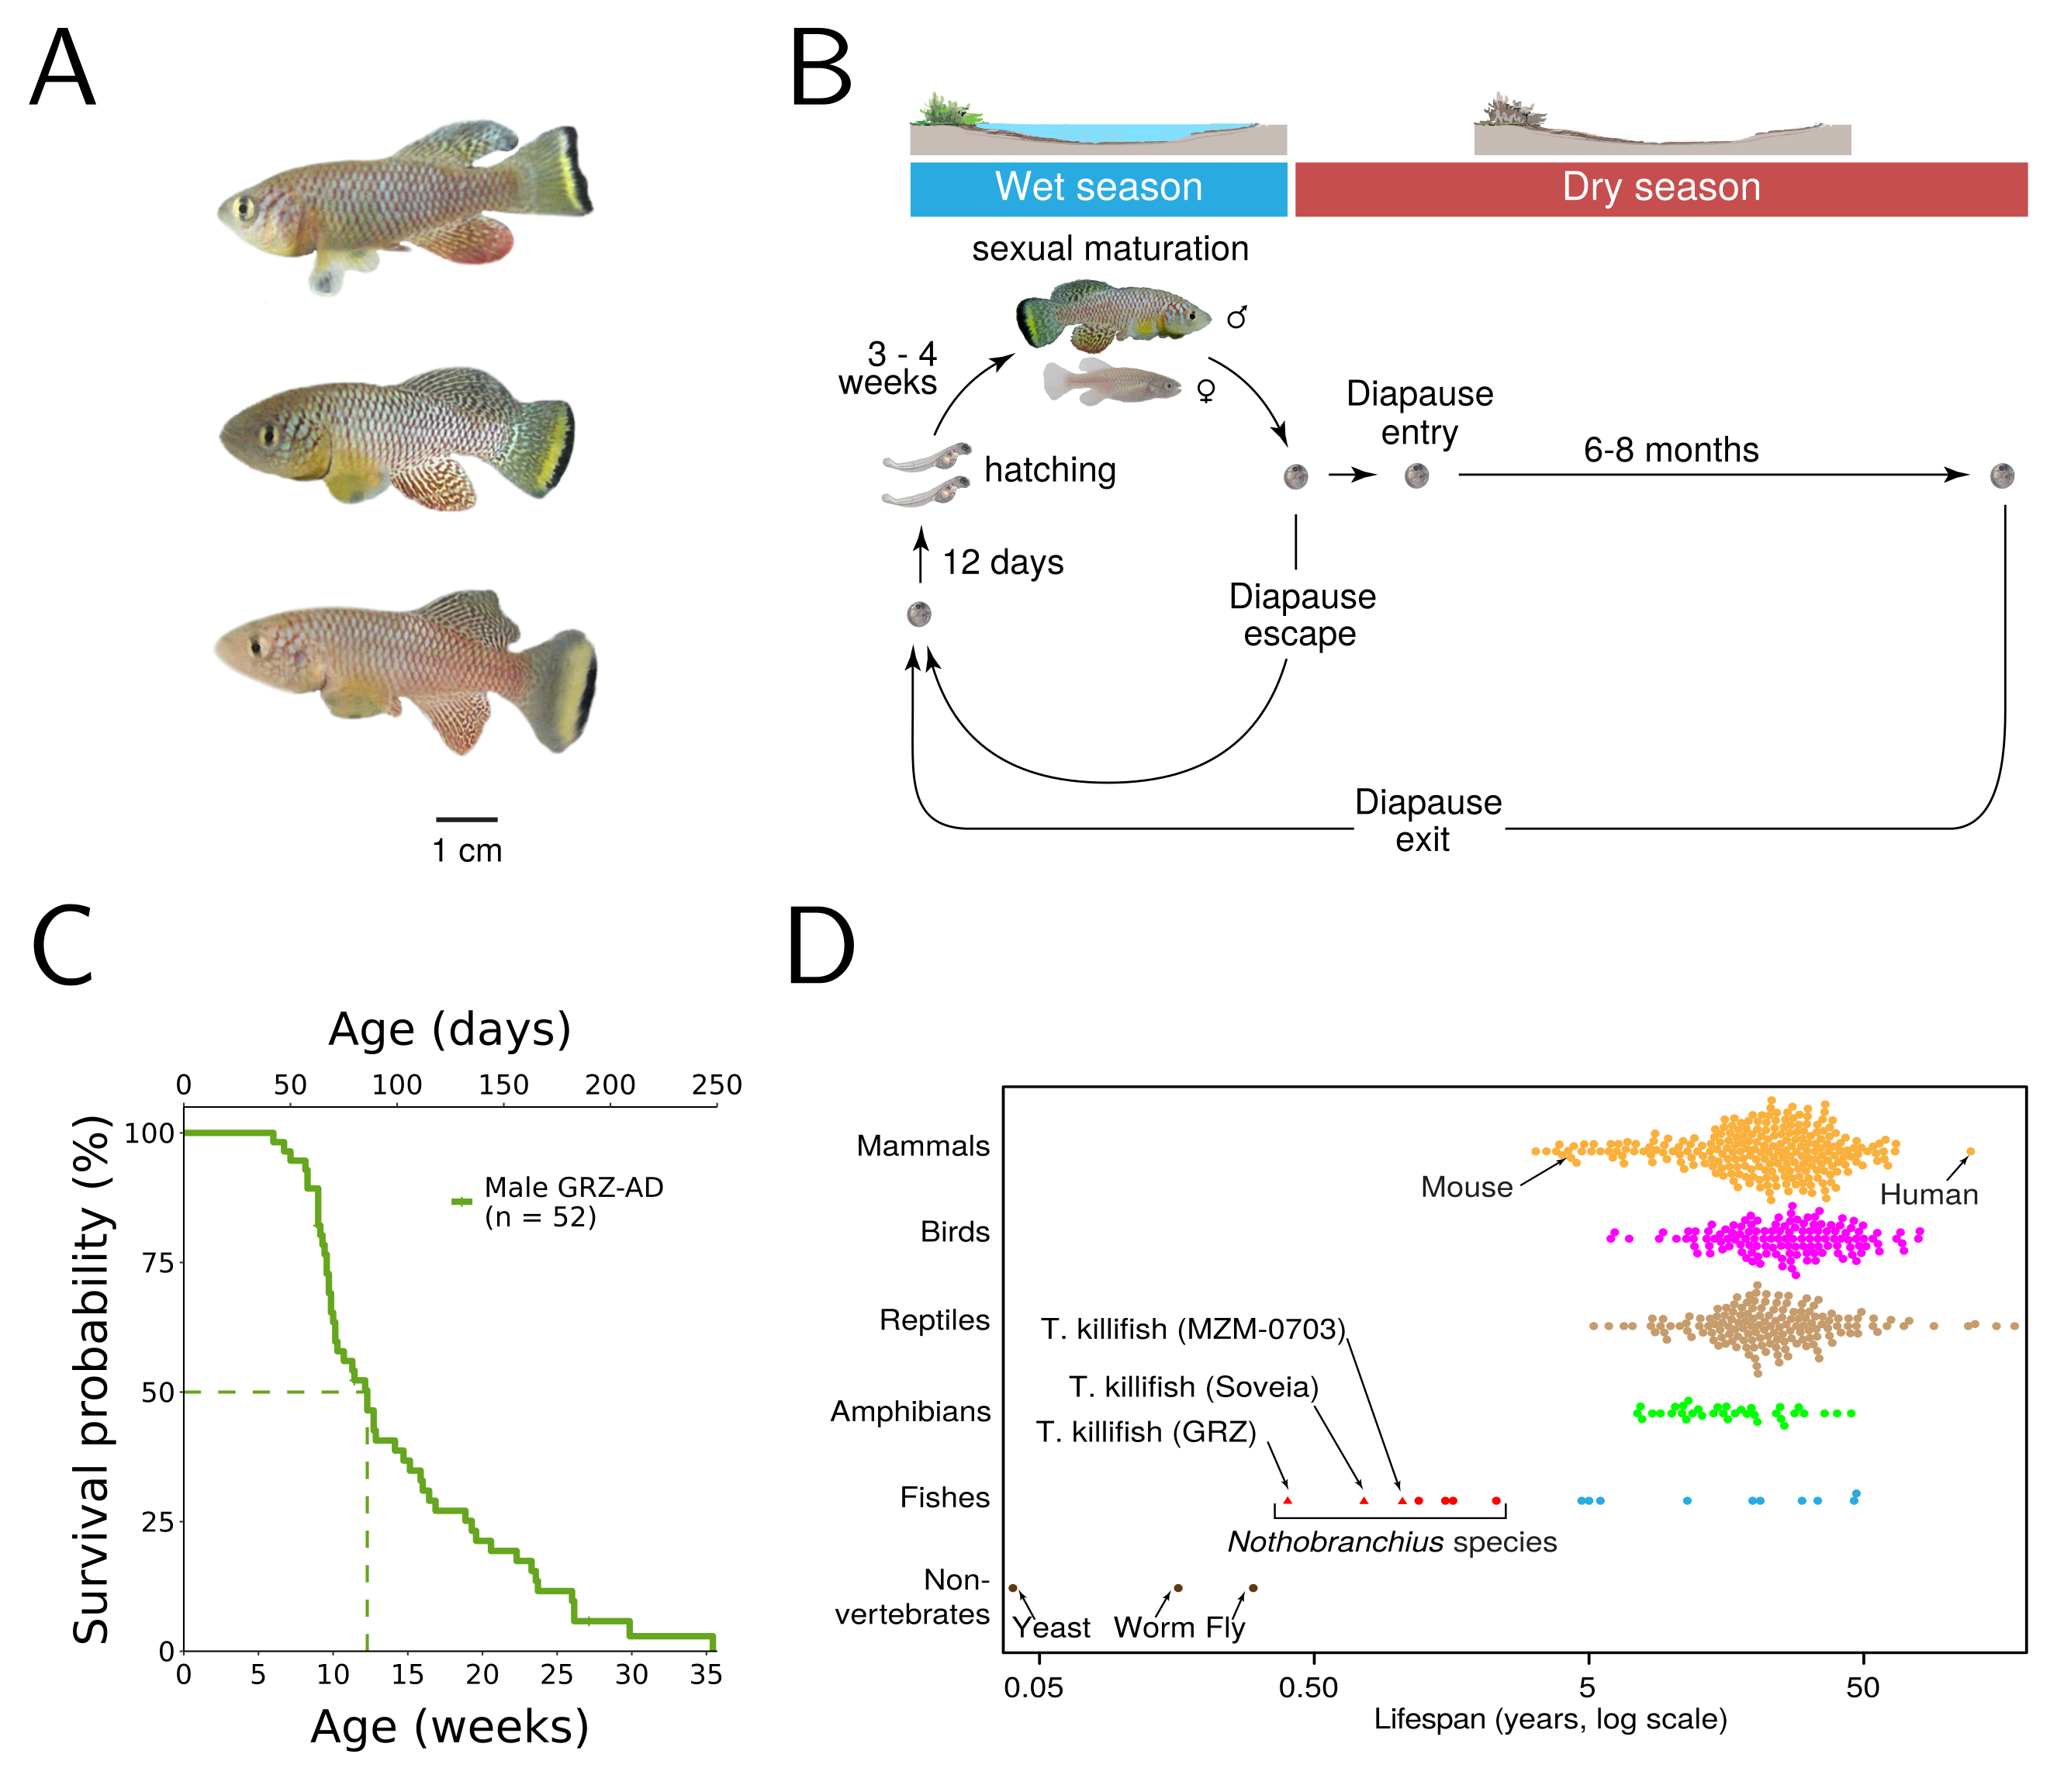
\includegraphics[width=0.95\textwidth]{_Figures/png_edited/intro-turquoise-killifish}
\caption{\textbf{The turquoise killifish as a model for vertebrate ageing:} (A) Photographs of male yellow-tailed turquoise killifish (\nfu).
(B) Life cycle of the turquoise killifish in its natural environment, showing hatching and breeding during the rainy season and embryo survival in diapause during the dry season.
(C) Example lifespan curve of short-lived GRZ-AD turquoise-killifish males, hatched in December 2016, with a median lifespan of roughly 12 weeks.
(D) Comparison of turquoise-killifish maximum lifespan (red triangles) to other vertebrate species, demonstrating the extremely short lifespan of \Nfu compared to other vertebrates. (A), (B) and (D) adapted from \parencite{valenzano2015genome}, Figure 1.}
\end{figure}